\chapter[2022 August]{August 2022}

\section[2022/08/01]{Monday, 01 August 2022}
\subsection{First draft of literature review for first-semester report.}

With an increase in the proliferation of powerful personal computing hardware it has become feasible to create augmented reality applications that merge together virtual objects and a user’s environment. Similarly, modern computer systems are capable of performing real-time machine learning inference on a large range of inputs and returning meaningful results – this has led to the advent of human-control inputs to computers like hand gesture control. 

These two subfields, augmented reality and gesture control can be combined to give a user a natural and intuitive control mechanism for interactive and visual applications. The literature is studded with examples of applications that use this combination of technologies such as \textbf{Australiaspiders} who utilize augmented reality and gesture control to treat agoraphobia using an interactive augmented reality application as well as \textbf{markerlessar} who use gesture input to select, shrink and zoom in on virtual objects as well as take in gesture volume controls for a music application.  COORDINATE SYSTEM

Hand gesture control can be considered as the two sequential problems of hand pose estimation and gesture recognition based on the hand pose predicted. Gesture recognition is most often performed using machine learning approaches such as support vector machines,  naïve-bayes classifiers and convolutional neural networks as is done in \textbf{Indiansign language} for the recognition of Indian sign language based on hand coordinate input. It can also be accomplished by extracting features from the input image using Gabor Wavelet Transforms and gradient local-autocorellation and then providing those features to a multi-layer perceprtron or K-nearest neighbors system such as in \textbf{combinedsignlanguage} to recognize sign language. The complexity of the algorithm required in gesture recognition depends on the static or dynamic nature of the input gestures as well as the diversity of input gestures.

What is apparent from the literature however is that the main challenge of gesture recognition is first acquiring an estimation of the user’s hand pose from camera input –solutions to this problem have been proposed and implemented since the 1990s. These early solutions \textbf{handclassicalapproach} relied on classical approaches to hand pose estimation such as using The Continuously Adaptive Mean Shift algorithm to recognize very high or low saturation of image pixels to segment a hand from its background and then using a curvature-based least-square fitting algorithm for detecting the contours of the hand such as fingertips. However, with the advent of modern computing power alluded to earlier and the rise of deep learning, the literature has been saturated with machine learning approaches to hand pose estimation. 

A state-of-the-art hand-tracking application created by Google dubbed Mediapipe Hands Google \textbf{mediapipe}, uses a series of convolutional neural networks to train a palm detector and hand landmark model on the cropped image of a hand to output hand landmark coordinates. The system runs in real-time on mobile devices and is trained using real images of hands as well as synthetic hand models. Similarly, \textbf{deepcnn} uses a deep convolutional neural network with just convolutional and pooling layers to output three-dimensional joint locations for a hand based on webcam input. This is why the literature often refers to hand pose estimation also as hand joint-regression. \textbf{handposergbcamera} employs a similar architecture to predict joint locations by first using a convolutional neural network to detect and segment the hand using a box prediction system reminiscent of YOLO9000 \textbf{yolo9000}, and then regress the joints of the hand using a large convolutional neural network based on the architecture of RESNet50 \textbf{resnet50}.

Alternatively, there are implementations of hand pose estimation that make use of not only standard RGB web camera input but also of depth camera input. This depth input is often modified in an intermediate transform such as a heatmap to show where each joint of the hand is likely to be and regresses the location of the joints from this intermediate layer. This is the approach taken in \textbf{poseguidedcnn} where a convolutional neural network regresses joing locations from feature regions which are themselves extracted from feature heatmaps created by depth image input. \textbf{cnnfinetuning} and \textbf{depthheatmaps} also make use of heatmaps of joint coordinates and finetuning algorithms later to output joint locations based on the intermediate layers and a number of transforms. 

\textbf{handposeocclusions} develops an architecture that involves calculating a skeleton-difference loss network to accept depth images as input, segment a hand based on the depth data and intermediate position score map system and then predict hand joints using convolutional layers and a 101-layer recurrent neural network. This implementation is developed to be robust to occlusions of the hand by objects held in the hand as well. Hand pose estimation is a subfield itself of full-body pose estimation which is a problem solved by \textbf{deeppose}, which takes advantage of a hierarchial progression of increasingly-fine-grained pose regressors for the joints of a whole body and is comprised at its core layer of simple convolutional layers stacked after each other. 

It is evident that the advent of deep learning has yielded a large number of machine learning approaches to not only hand pose estimation but also full-body pose estimation and that the extensive use of convolutional neural networks is the modern approach most preferred in academia. This is due to the ease of not having to implement detailed representations of low-level hand shapes, patterns and methods of finding them but rather instead training a machine learning system to identify and learn these low-level abstractions using vast amounts of training data and machine learning architectures such as the convolutional neural network.

In conclusion, to implement a system that can perform hand gesture control of a virtual object in augmented reality it is evident that the preferred approach in the literature for such a task is to use a deep-learning approach to regress hand joint coordinates from either a depth or standard RGB camera. Gesture recognition can either be performed by machine learning approaches or by classical calculations depending on the complexity of the required gestures. Augmented reality and the combination of virtual reality objects with real-world objects can create immersive and useful applications when a suitable input camera is used to capture video and depth data about the environment. A system will thus be developed that can accept user gesture input using a deep-learning approach and then translate that gesture into meaningful instructions for a virtual object present in an augmented reality scene that is tied together using a global coordinate system and presents realistic physics and interactions between the objects based on a simulated collision avoidance system.

\subsection{OpenGL Movement API}

The objective of this work session is to create a small API for converting normalized xyz world coordinates into OpenGL coordinates so that the virtual object and real world pixel coordinates can be compared. This is accomplished by setting an original 0,0,0 coordinate for the virtual object when the program is initialized and updating it based on the passed in coordinates and the glTranslatef OpenGL command. Since the display window is set to be 800x600px the glTranslate method can take in a maximum of 8.0 and 6.0 for the x and y parameters respectively. Pictured in \FigRef{fig:opengl_cube_coordinate_system} is the cube at world coordinate (0,0) and the result of moving it there with gesture input provided by the mediapipe library.

\begin{figure}[h]
    \centering
    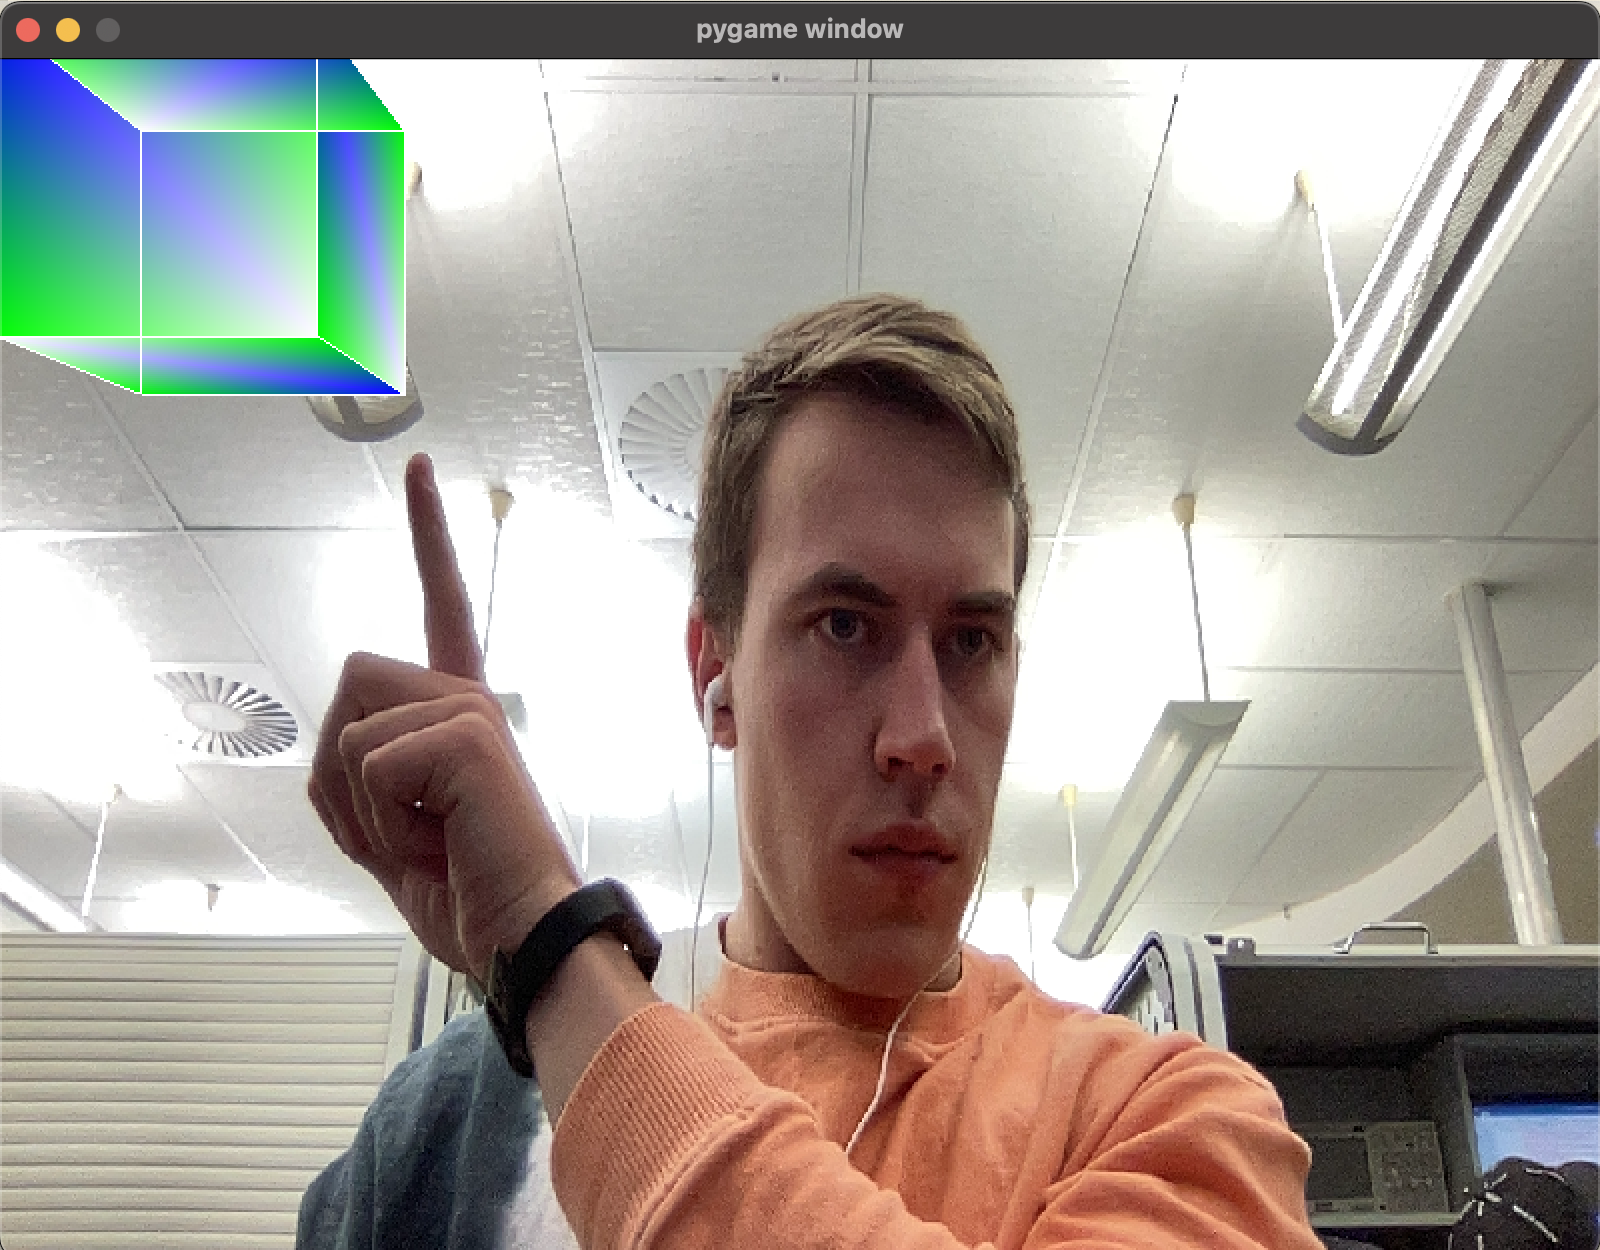
\includegraphics[width=0.7\linewidth]{figures/opengl_cube_coordinate_system.png}
    \caption{OpenGL virtual object at world coordinates 0,0.}
    \label{fig:opengl_cube_coordinate_system}
\end{figure}

\section[2022/08/02]{Tuesday, 02 August 2022}
\subsection{Neural network convolutional layers}

The aim of the work session today is to get multiple convolutional layers working with each other in the layers version of the convolutional neural network. This involved refactoring code so that output from a previous convolutional layer could be accepted as input to the next one - this mainly consisted of changing the order of for loops and iterations through the dimensions of the filter arrays and outputs so that multiple filters with x and y components with multiple channels $filters[numFilters][x][y][numChannels]$ could match with other variables like the convolutional loss gradient from following layers $convolution\_gradient[numFilters][x][y][numChannels].$

\section[2022/08/03]{Wednesday, 03 August 2022}

\subsection{More training data for gesture classifier}

The aim of today's work session is to build up a large dataset of hand coordinates and their corresponding images for better training.

The dataset can be found in the repo in the "handcoordstrainingdata" folder. It was attempted to train the network on this data but it took over an hour for just 5 epochs. Attempts were made to shrink the input images to dimensions of just 20x15 but at this resolution not enough data remained for good generalization. Preprocessing was introduced in the form of the edge detection filter and convolution previously used in experimentation to detect the edges of objects using the Kinect sensor. This made the data much simpler and stripped away a lot of unnecessary background information and as of this writing training is still ongoing. It is hypothesized that in the final implementation of the system, it is going to be essential to perform preprocessing in this manner if the network is going to run in any efficient timeframe. Additionally, developing a hand segmentation algorithm or hand location algorithm would also be highly helpful and in-line with the industry-leading approach Mediapipe which does this to ensure that most of the learning capability of the network goes towards recognising a hand and not dealing with background information. \\

The industry standard activation function is the Relu function but using it in the place of the sigmoid function currently used gives garbage output from the CNN and a static epoch error rate. Perhaps the outputs of various layers need to be normalized or simplified to use this function but getting this working is a priority as it brings the architecture of the system in-line with known working solutions and is estimated to dramatically increase training and inferrence time as certain neurons and weights are saturated when they do not provide helpful information to the network. Additionally, implementing dropout regularization is a future goal as well.


\section[2022/08/04]{Thursday, 04 August 2022}

\subsection{Kinect Segmenting Prototyping And Keras Gesture learning}

The aim of the work session today is to experiment with using the depth values from the Kinect sensor for segmenting images and to use Keras to attempt to build a small gesture classifier using the same training data provided to the layers neural network developed from first principles.

The results of the image segmentation based on the Kinect depth data can be seen in \FigRef{fig:kinect_segment1} and \FigRef{fig:kinect_segment2}. The Kinect returns depth values from 0-2048 with values closer to the sensor being labelled closer to 0. With a threshold in place here to only display the pixel values where the corresponding depth value is less than 150 a segmentation algorithm can be created that only displays those things close to the sensor. This is potentially valuable in removing excessive background noise or information from processing. Additionally, it confirms that the Kinect sensor can only determine depth values from about 50cm away as any closer yields noise values.

\begin{figure}[h]
    \centering
    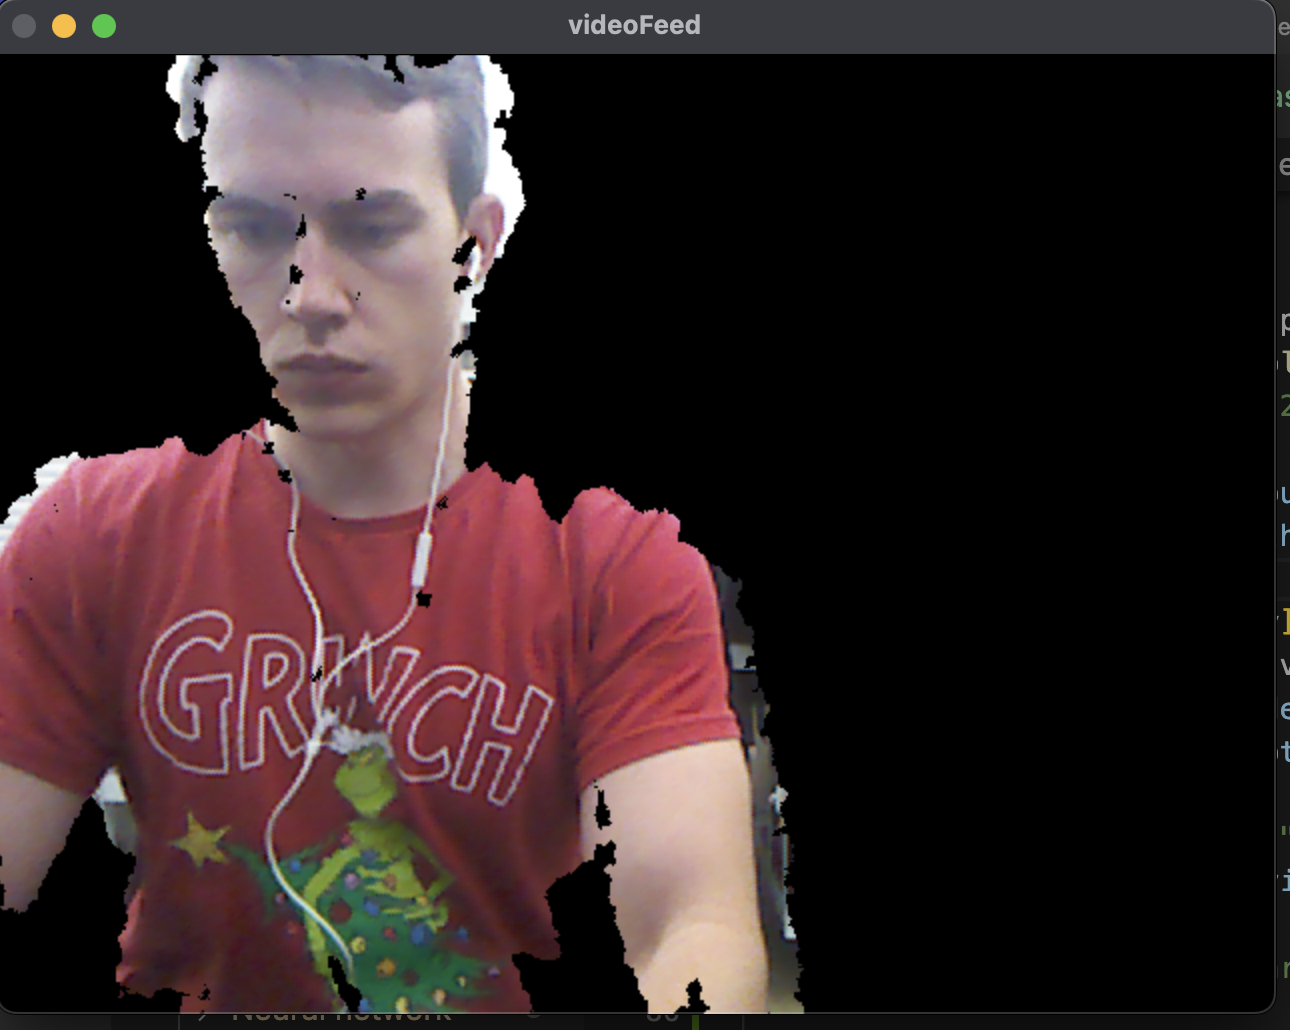
\includegraphics[width=0.7\linewidth]{figures/kinect_segment1.png}
    \caption{Segmenting an image based on the Kinect depth data}
    \label{fig:kinect_segment1}
\end{figure}

\begin{figure}[h]
    \centering
    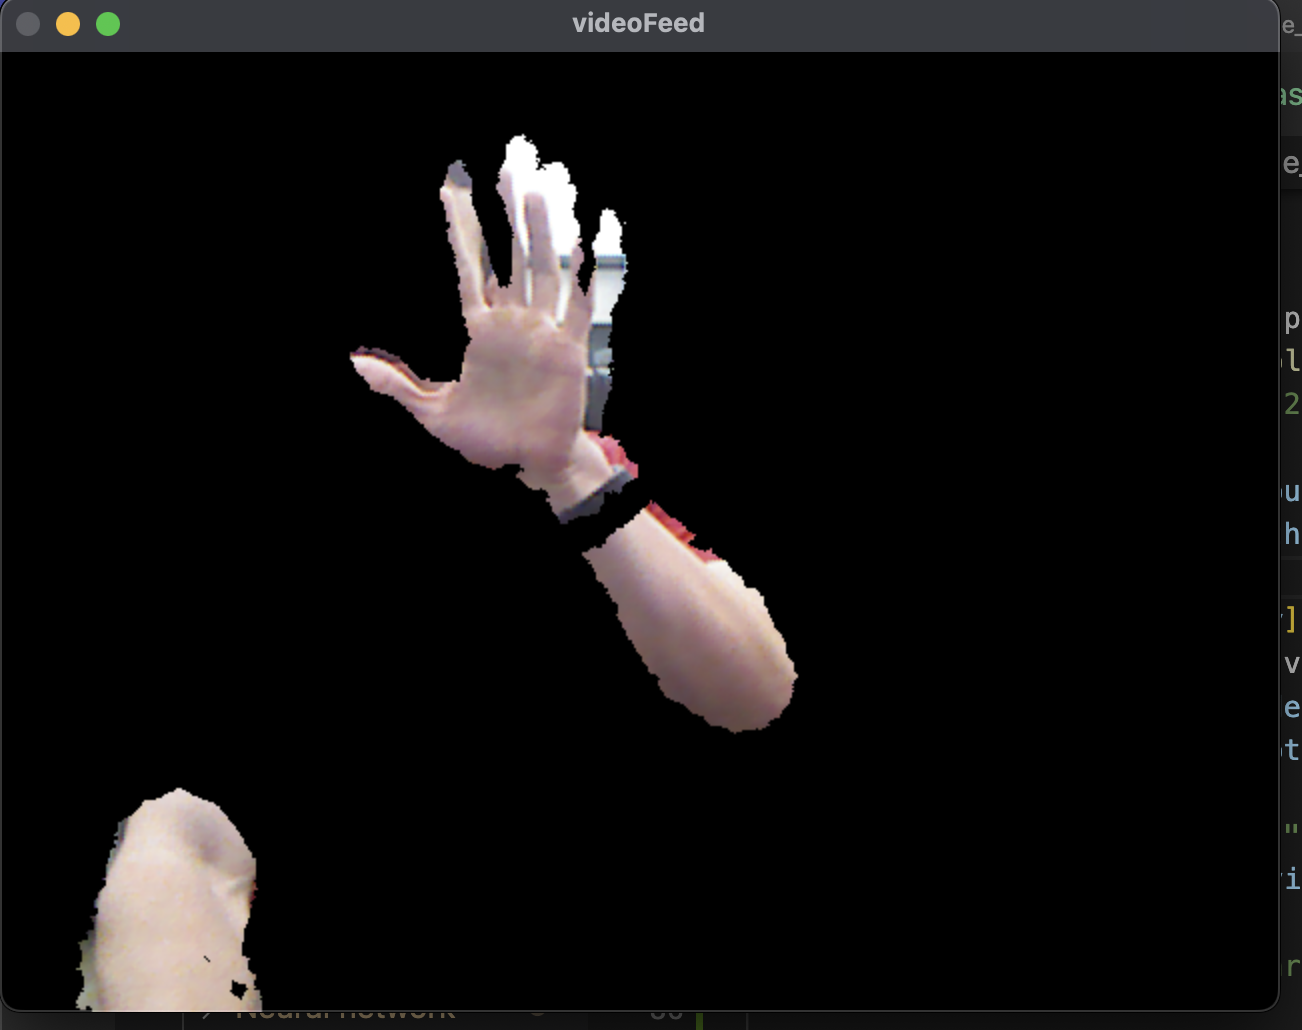
\includegraphics[width=0.7\linewidth]{figures/kinect_segment2.png}
    \caption{Segmenting an image based on the Kinect depth data}
    \label{fig:kinect_segment2}
\end{figure}

TeachableMachine and Keras was used to build a small fist/open hand classifier and the model downloaded and examined - only sequential or "hidden" layers were used and could accurately classify the data found in gesturetrainingdata. Removing the convolutional layers from the network also allowed the first principles implementation to classify these images correctly as visible in \FigRef{fig:layers_gesture_predictor1} and \FigRef{fig:layers_gesture_predictor1}. The network is definitely overfitted on the training data but it is a good first step in recognising gestures using webcam input.

\begin{figure}[h]
    \centering
    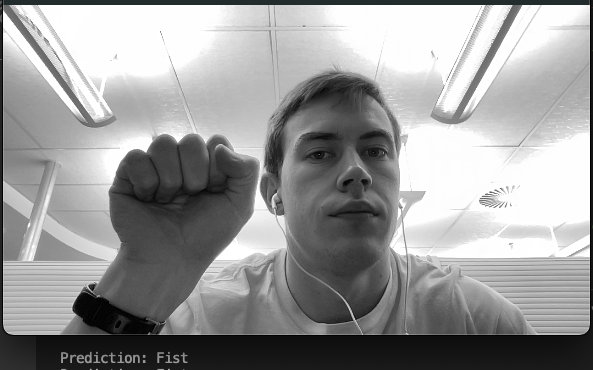
\includegraphics[width=0.7\linewidth]{figures/layers_gesture_predictor1.png}
    \caption{First principles open/closed hand predictor}
    \label{fig:layers_gesture_predictor1}
\end{figure}

\begin{figure}[h]
    \centering
    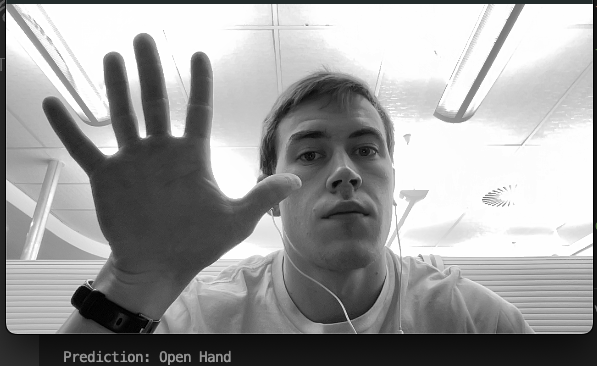
\includegraphics[width=0.7\linewidth]{figures/layers_gesture_predictor2.png}
    \caption{First principles open/closed hand predictor}
    \label{fig:layers_gesture_predictor2}
\end{figure}

Thus it is hypothesized that something is wrong with the convolutional layers and mathematics of the first principles implementation as a basic image classification task can be accomplished using just hidden and output layers.


\section[2022/08/05]{Friday, 05 August 2022}

\subsection{First Semester Report Submitted}

The first semester report was submitted and the final version of the literature review - with correct referencing, is including below.

With the increase in the proliferation of powerful personal computing hardware it has become feasible to create augmented reality applications that integrate virtual objects with a user’s physical environment. Similarly, modern computer systems can perform real-time inference on a large range of alternative inputs and return useful results – this has led to the advent of human-control inputs to computers like hand gesture control. \\

These two sub-fields - augmented reality and gesture control, can be combined to give a user a natural and intuitive control mechanism for interactive and visual applications. The literature is studded with examples of applications that use this combination of technologies, such as Billinghurst \cite{Australia_spiders} who utilizes a Microsoft Kinect depth and RGB camera to treat agoraphobia by creating virtual spiders that the user can interact with using their hands in an augmented reality application. Baldauf \cite{markerless_ar} uses gesture input from a mobile phone camera to select, shrink and zoom in on virtual objects presented in the environment as well as to recognize gesture volume controls for a music application. \\

The ability to locate virtual objects in the context of the real-world environment in an augmented reality application is important if realistic interaction is to take place. Kato \cite{ar_tabletop} implements a tabletop augmented reality application for handling small virtual shapes that relies upon a global coordinate system and paper tracking fiducials placed on the tabletop to give both virtual objects and real-world objects their coordinates in the global coordinate system and then be able to control virtual object movement and behavior accordingly. Similarly, Buchmann \cite{fingartips} uses a world coordinate system in an urban planning augmented reality application that tracks the position of virtual objects as well as the user’s hand and current gesture to determine if an object should be grasped, moved or released at any given time. This also allows for collision avoidance as the same coordinate system is shared by all objects – real or virtual. \\

These applications receive hand gestures as input and hand gesture control itself can be considered as the two sequential problems of hand pose estimation and gesture recognition based on the hand pose predicted. Gesture recognition is most often performed using machine learning approaches such as support vector machines, Naïve-Bayes classifiers and convolutional neural networks as by Ahmed \cite{indian_sign_language} for the recognition of Indian sign language based on hand coordinate input. It can also be accomplished by extracting features from the input image using Gabor Wavelet Transforms and gradient local-auto correlation and then providing these features to a multi-layer perceptron or K-nearest neighbors system such as by Sadeddine \cite{combined_sign_language} to recognize sign language. The complexity of the algorithm required in gesture recognition depends on the static or dynamic nature as well as diversity of the input gestures. \\

What is apparent from the literature, however, is that the main challenge of gesture recognition is first acquiring an estimation of the user’s hand pose from camera input – solutions to this problem have been proposed and implemented since the 1990s. These early solutions \cite{hand_classical_approach} relied on classical approaches to hand pose estimation such as using The Continuously Adaptive Mean Shift algorithm to recognize very high or low saturation of image pixels to segment a hand from its background and then using a curvature-based least-square fitting algorithm for detecting the contours of the hand such as fingertips. An alternative to hand pose estimation is to use a physical glove with fiducial markers on it as used by Buchmann \cite{fingartips} to detect the position of a user’s hand in space. However, with the advent of modern computing power and the rise of deep learning, the literature has been saturated with machine learning approaches to hand pose estimation that require none of the special hardware or highly specific algorithms that previous implementations required.  \\

A state-of-the-art hand-tracking application created by Google - dubbed Mediapipe Hands \cite{mediapipe_hands}, uses a series of convolutional neural networks to train a palm detector and hand landmark model to output coordinates of hand landmarks. The system runs in real-time on mobile devices and is trained using real images of hands as well as synthetic hand models. Similarly, Qing \cite{deep_cnn} uses a deep convolutional neural network with just convolutional and pooling layers to output three-dimensional joint locations for a hand based on webcam input. This is why the literature often refers to hand pose estimation as hand joint-regression. Gomez-Donoso \cite{hand_pose_rgb_camera} employs a similar architecture to predict joint locations by first using a convolutional neural network to detect and segment the hand using a box prediction system reminiscent of the YOLO9000 architecture \cite{yolo_9000}, and then regress the joints of the hand using a large convolutional neural network based on the RESNET50 architecture \cite{resnet_50}.  \\

Alternatively, there are implementations of hand pose estimation that also make use of depth camera input. This depth input is often modified in an intermediate transformation such as a heatmap to show where each joint of the hand is likely to be and regresses the location of the joints from this intermediate layer. This is the approach taken by Chen \cite{pose_guided_cnn} where a convolutional neural network regresses joint locations from feature regions which are themselves extracted from feature heatmaps created by depth image input. Ding \cite{cnn_finetuning} and Ge \cite{depth_heatmaps} also make use of heatmaps of joint coordinates and subsequent fine-tuning algorithms to output joint locations based on the intermediate layers.  \\

% Wu \cite{hand_pose_occlusions} develops an architecture that involves calculating a skeleton-difference loss network to accept depth images as input, segment a hand based on the depth data and intermediate joint position score map created, and then predicts hand joints using convolutional layers and a 101-layer recurrent neural network. This implementation is developed to be robust to occlusions of the hand by objects held in the hand as well. Hand pose estimation itself is a sub-field of full-body pose estimation which is a problem solved by Toshev \cite{deep_pose}, which takes advantage of a hierarchical progression of increasingly-fine-grained pose regressors for the joints of a whole body and is comprised at its core of simple convolutional layers stacked after one another.  \\

It is evident that the advent of deep learning has yielded a large number of machine learning approaches to hand pose estimation and that the extensive use of convolutional neural networks is the modern approach most preferred in academia. This is due to the ease of not having to implement detailed representations of low-level hand shapes, patterns and methods of identifying these features in input imagery but rather instead training a machine learning system to identify and learn these low-level abstractions using vast amounts of training data and machine learning architectures such as the convolutional neural network. \\

In conclusion, to implement a system that can perform hand gesture control of a virtual object in augmented reality it is evident that the preferred approach in the literature for such a task is to use a deep-learning architecture to regress hand joint coordinates from either a depth or standard RGB camera input. Gesture recognition can either be performed by machine learning approaches or by classical calculations depending on the complexity of the required gestures. Augmented reality and the combination of virtual reality objects with real-world objects can create immersive and useful applications when a suitable input camera is used and a shared coordinate system is established to track both virtual and real objects and prevent collisions between them. A system will thus be developed that can accept user gesture input using a deep-learning approach and then translate that gesture into meaningful instructions for a virtual object present in an augmented reality scene that presents realistic interactions between the objects and uses a global coordinate system to prevent object collisions. \\

\subsection{Fixing Dying Relu Problem}
The use of the relu function as the activation function has long given errors in the first principles implementation as after a single epoch of training the error remained constant and no learning could take place. This was hypothesized to be because of a dying relu problem where the output of a relu function is almost 0. The output of each layer and the current value of the hidden and output weights were printed to the network details textfile and upon examination it seemed that the weights were initially set and then never really changed again. Changing the weight initialization to much smaller values, like -0.1 to 0.1, seemed to alleviate this problem but the network shortly converged to the same epoch error and stayed there. Research was done into the effects of weight initialization, batch normalization and regularization and these operations may have to be implemented in order to get the relu activation function working correctly. \\

\subsection{Retraining of basic gesture classifier with convolutional network}

It was attempted to train the network using one convolutional layer and one hidden layer to predict the open/closed hand gestures. However, after 15 hours of training the learning was still ongoing on a 2020 Macbook Air M1 laptop. Alternative training approaches have to be considered if the project is to be completed on-time - at this rate of training it is infeasible to test different designs. The use of Google Colab notebooks was briefly investigated however since the first principles implementation doesn't use a GPU or TPU-optimized framework like Tensorflow or Pytorch the advantages of a GPU or TPU are wasted and the implementation actually ran slower than on the Macbook Air PC. 

\section[2022/08/05]{Friday, 05 August 2022}

\subsection{Brainstorming collision avoidance pipeline}

The training for the CNN to classify open/closed hand gestures is still ongoing.\\

In order to create realistic interactions between the virtual object and real-world objects it is going to be necessary to perform collision avoidance when attempting to move the virtual object. A proposed pipeline for this process is presented in \FigRef{fig:Proposed Collision Avoidance Algorithm}.

\begin{figure}[h]
    \centering
    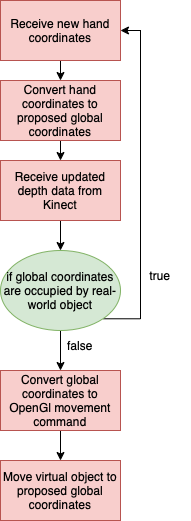
\includegraphics[width=0.2\linewidth]{figures/Proposed Collision Avoidance Algorithm.png}
    \caption{Proposed Collision Avoidance Algorithm.png}
    \label{fig:Proposed Collision Avoidance Algorithm}
\end{figure}

The training of the hand closed/open network was terminated after 20 hours and still an epoch error of over 40. Additional modifications to the network and training process are obviously necessary to achieve the desired performance. Specifically, segmenting the hand from the background is going to be a necessary step to remove complexity from the neural network and focus on classifying hand coordinates/gestures and not whole body shapes. This is what \cite{mediapipe_hands} did. Thus in the aim of building a hand detector the Ycbcr color space is used to experimentally interpret the values from a webcam, since skin hue color is a specific color and can be segmented from other colors - a computationally cheap way of identifying skin in an image. The Ycbcr color space is defined as " Y the luma component and CB and CR are the blue-difference and red-difference chroma components." A webcam image converted into this color space is presented in \FigRef{fig:Ycbcr_hands.png} and thresholding using the values of the color space is presented in \FigRef{fig:Ycbcr_segmentation}. Background colours similar to the colour of the hand provide background noise however it clearly segments the hand and face based on skin colour and is a promising approach for hand segmentation.

\begin{figure}[h]
    \centering
    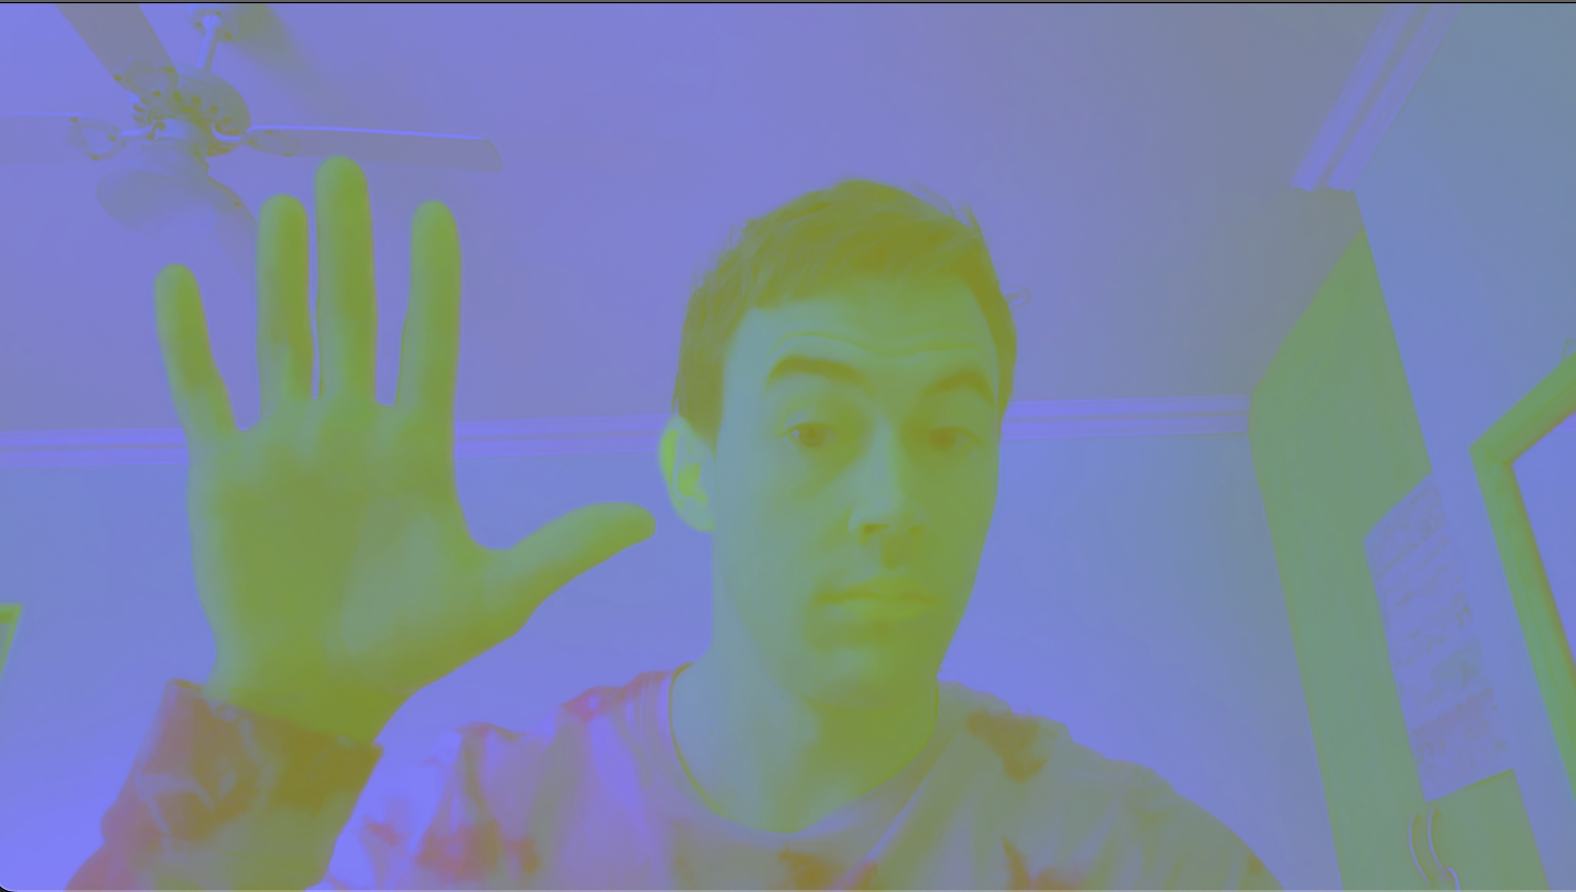
\includegraphics[width=0.7\linewidth]{figures/Ycbcr_hands.png}
    \caption{Ycbcr-encoded webcam image}
    \label{fig:Ycbcr_hands.png}
\end{figure}

\begin{figure}[h]
    \centering
    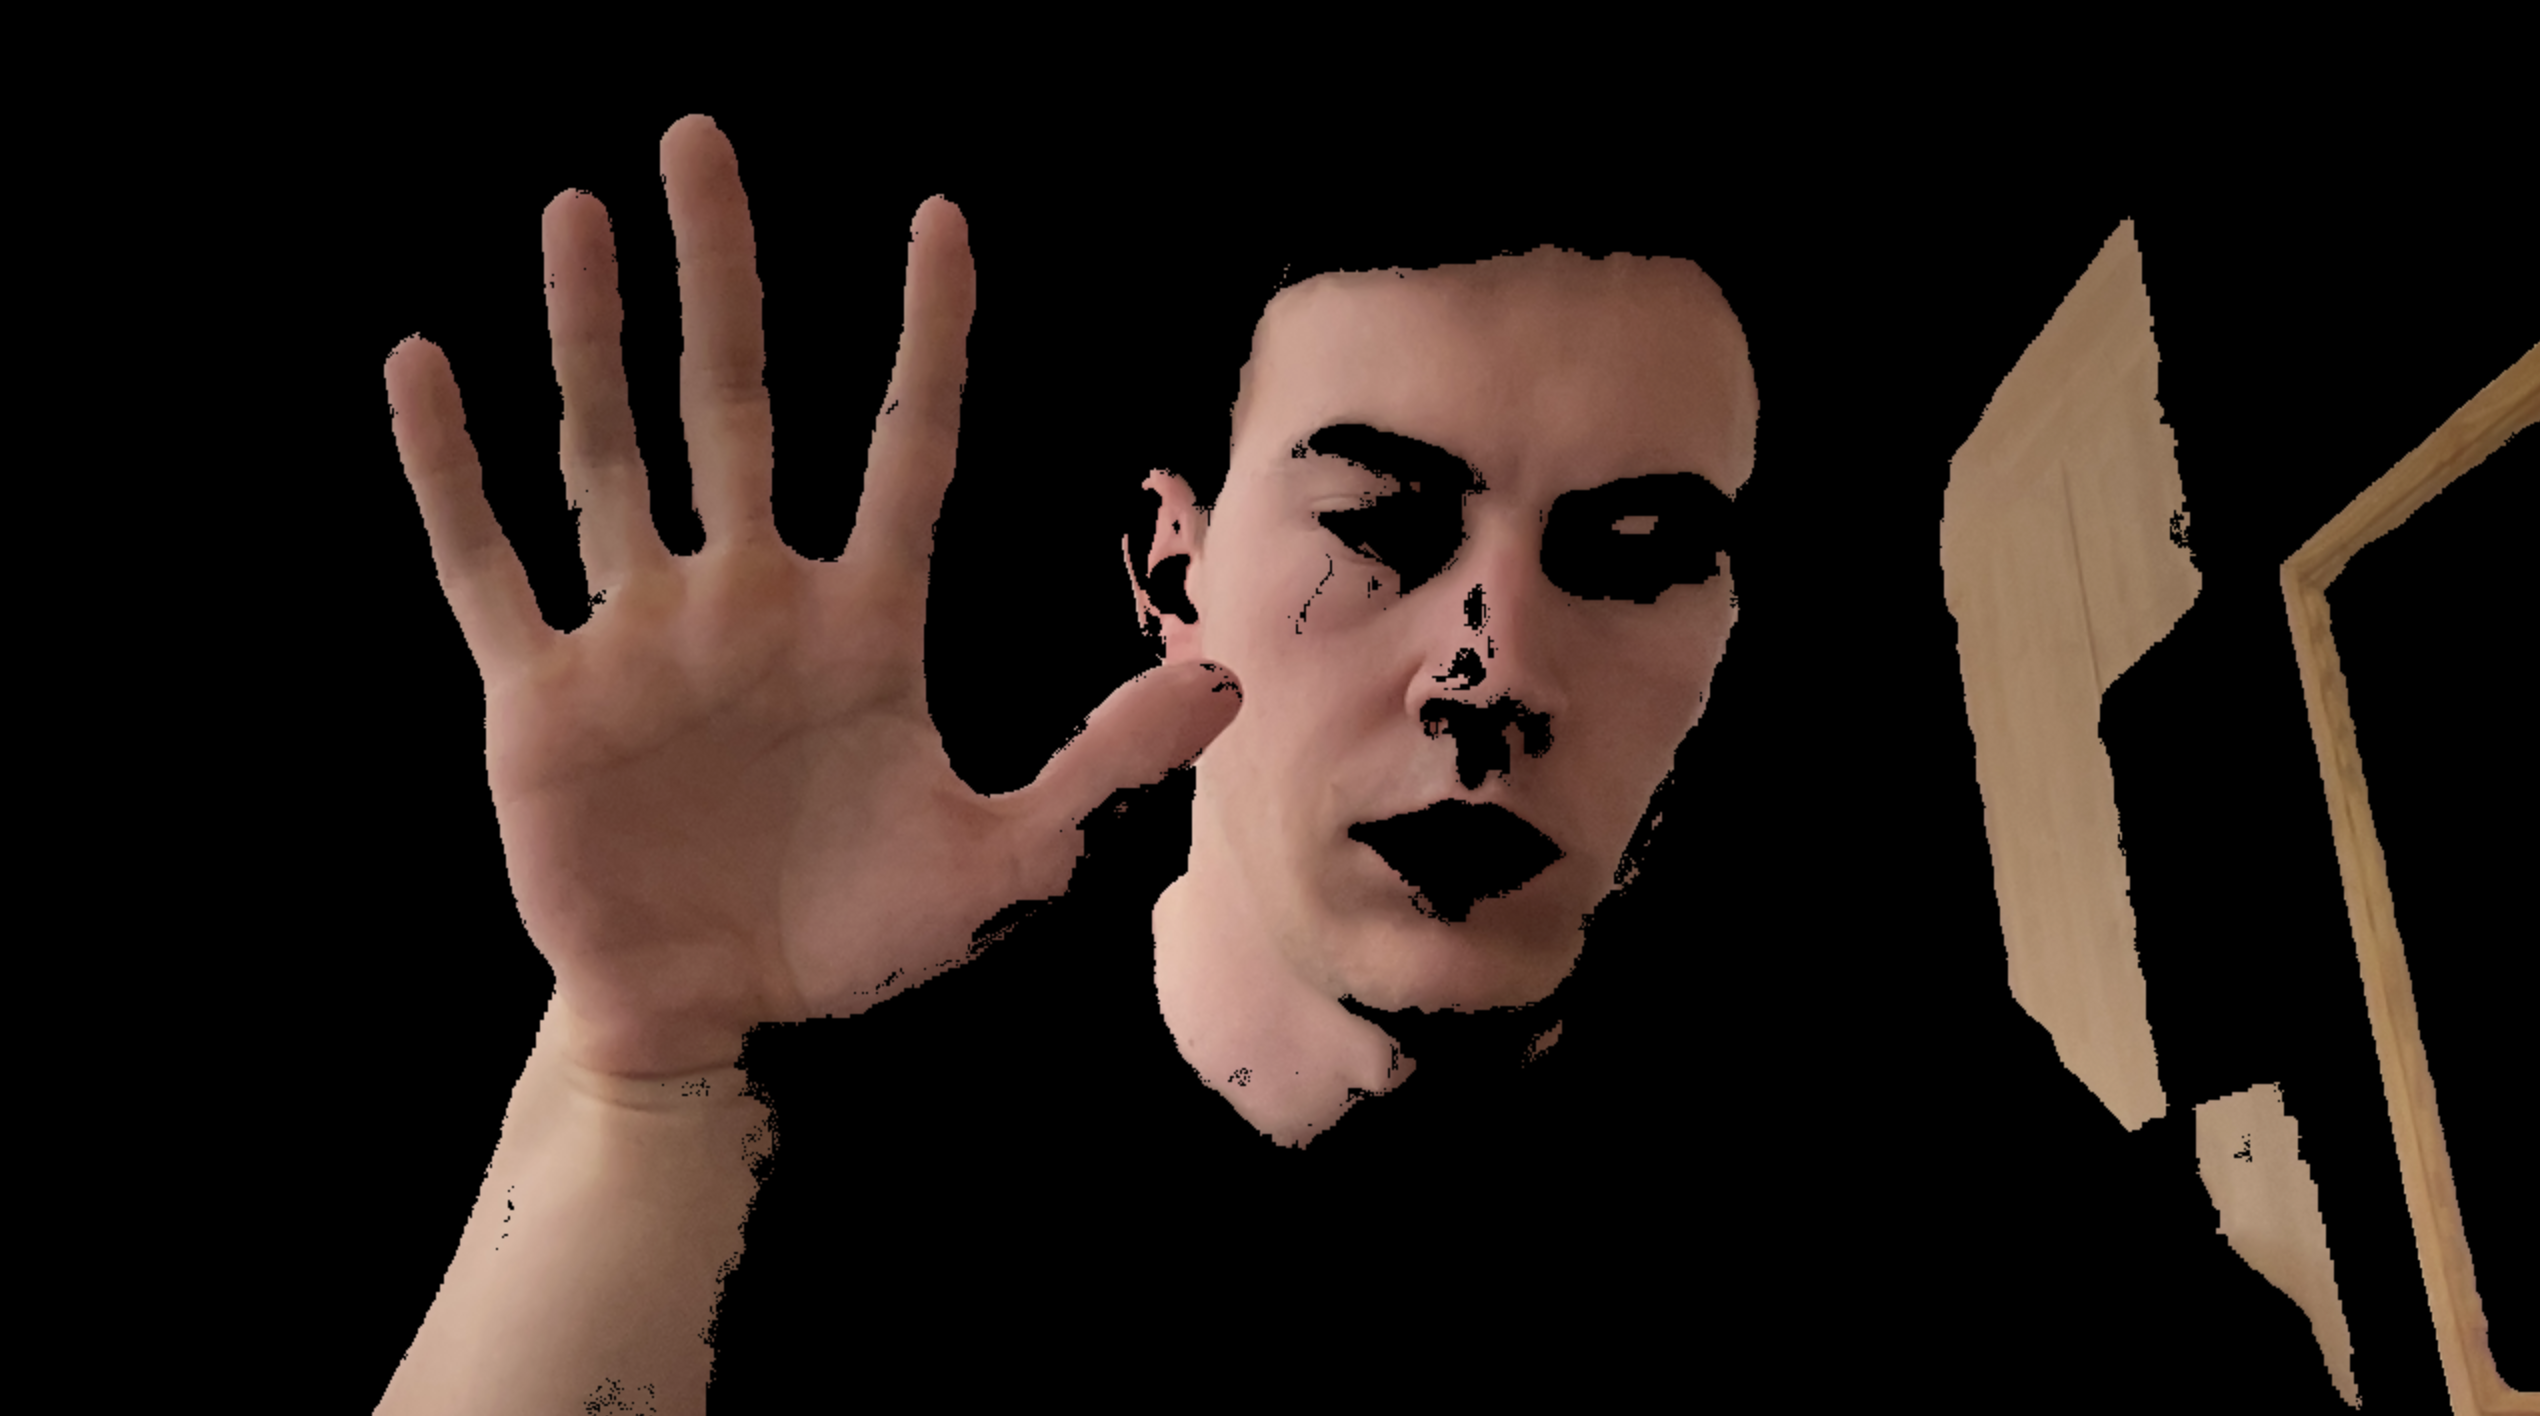
\includegraphics[width=0.7\linewidth]{figures/Ycbcr_segmentation.png}
    \caption{Ycbcr segmentation}
    \label{fig:Ycbcr_segmentation}
\end{figure}

\section[2022/08/09]{Tuesday, 09 August 2022}

\subsection{Brainstorming segmentation and more efficient algorithms}

Time was spent during this work session researching the Ycbcr color space further and experimenting with it. Several research papers combine color space and depth information in order to correctly segment hands from an image. The computational speed of searching through the entire depth and color arrays provided as input from cameras is very inefficient - using built-in Python functions such as array indexing with code like $result = np.where((array >2), array, 0)$ to perform thresholding on values smaller than 2 can drastically reduce runtime and improve performance. Produced in \FigRef{fig:handwritten_notes_9_aug} is the handwritten lab notes entry from today brainstorming algorithm processes and the thresholding pipeline for hand detection.

\begin{figure}[h]
    \centering
    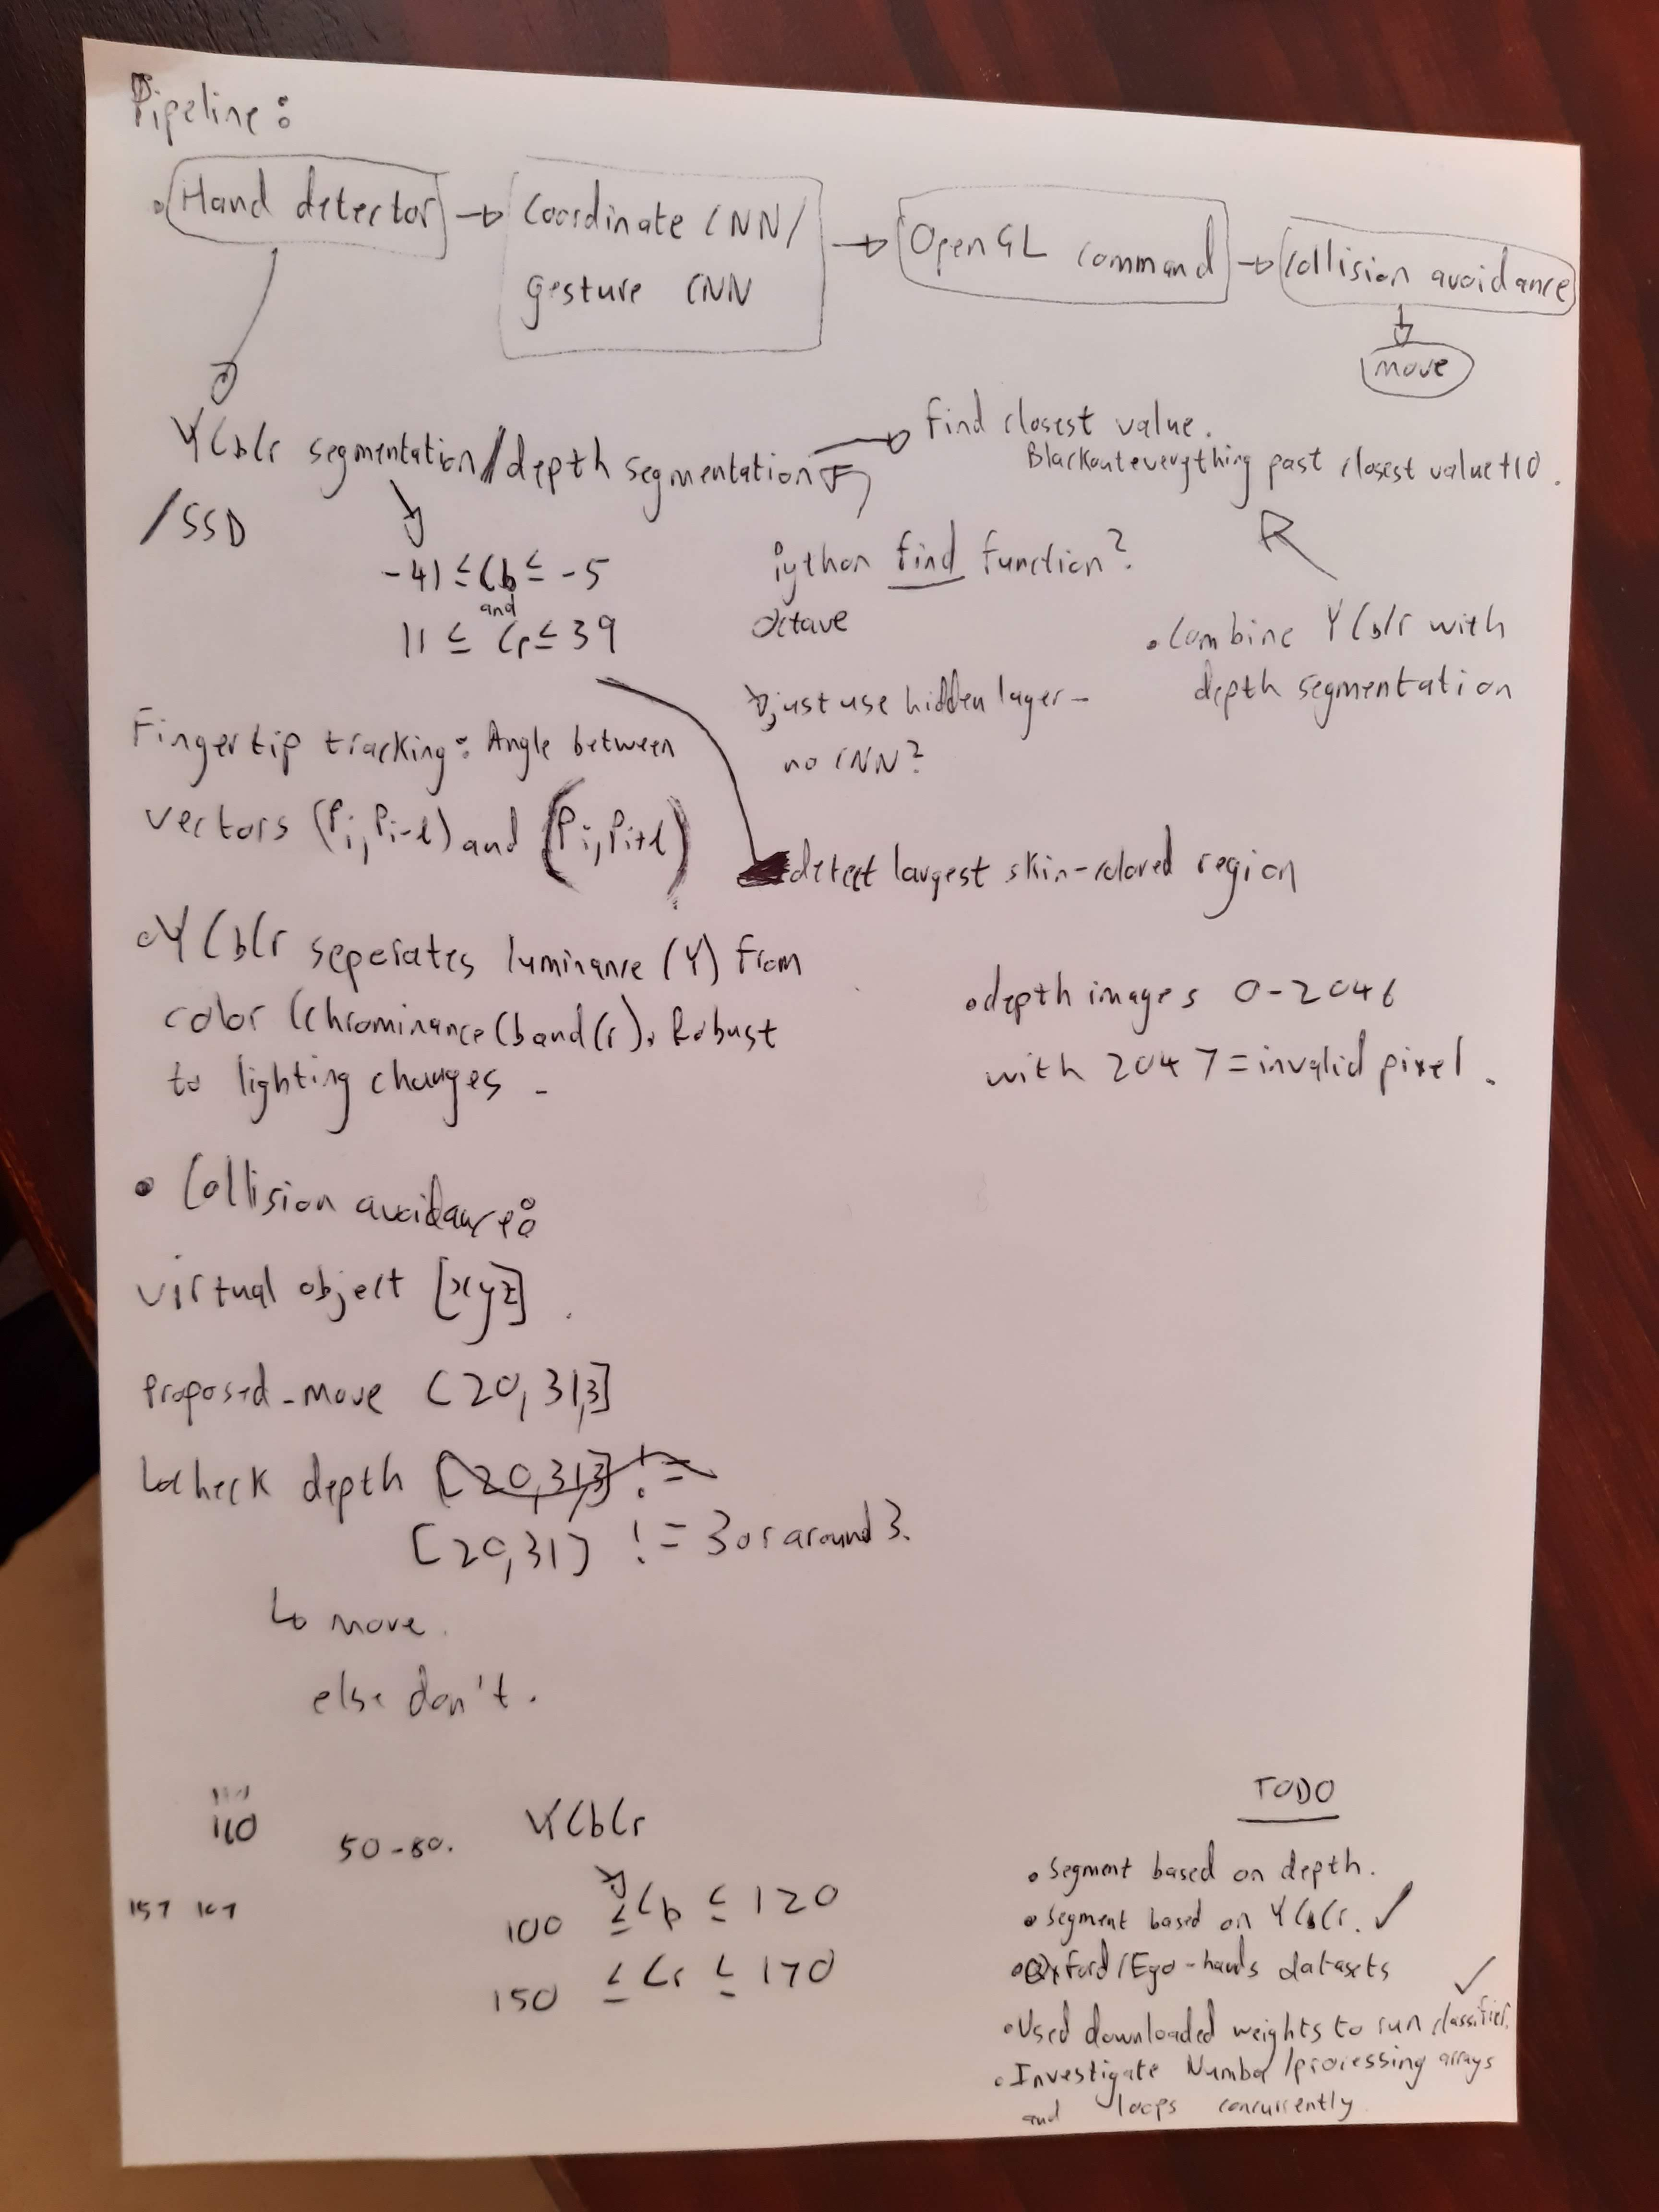
\includegraphics[width=0.7\linewidth]{figures/handwritten_notes_9_aug.jpg}
    \caption{Handwritten notes brainstorming color and depth segmentation}
    \label{fig:handwritten_notes_9_aug}
\end{figure}

\section[2022/08/11]{Thursday, 11 August 2022}

\subsection{Using the Keras and Tensorflow libraries to train networks}

The aim of this work session is to use Keras and Tensorflow to build a gesture recognition system.

In a meeting with Mr. Grobler on the Wednesday, 10 August 2022, the excessive slowness of training neural networks using the first principles implementation reported on earlier in this document was discussed. It was decided that it would be prudent to use an optimized library like Tensorflow to conduct the training of the gesture classifer neural network in order to speed up the process to tolerable wait times. This was agreed too not to be in violation of constructing all systems of the Project from first principles due to the actual implemented system (the gesture classifier and network) will still work with a first-principles forward-propagation implementation and no libraries. However using a library to obtain the correct weights of the network was deemed a fair use of existing tools since the goal of the project is not to build an end-to-end first principles machine learning pipeline but rather achieve the objective of real-time gesture recognition. Additionally, the first-principles implementation of the training and backpropagation process can be shown to work albeit slowly and discussed and compared to existing libraries in the final report. \\

Thus learning commenced yesterday on August 9, 2022 and experimentation with the Keras and Tensorflow libraries began. This resulted in the construction of a reliable open-hand/fist classifier using the architecture shown in \FigRef{fig:tensorflow_open_hand_fist_arch} with good accuracy as shown in  \FigRef{fig:tensorflow_open_hand_fist_accuracy}. The output of the system on live webcam input is shown in \FigRef{fig:tensorflow_open_hand_fist_prediction1} and \FigRef{fig:tensorflow_open_hand_fist_prediction2}.

\begin{figure}[h]
    \centering
    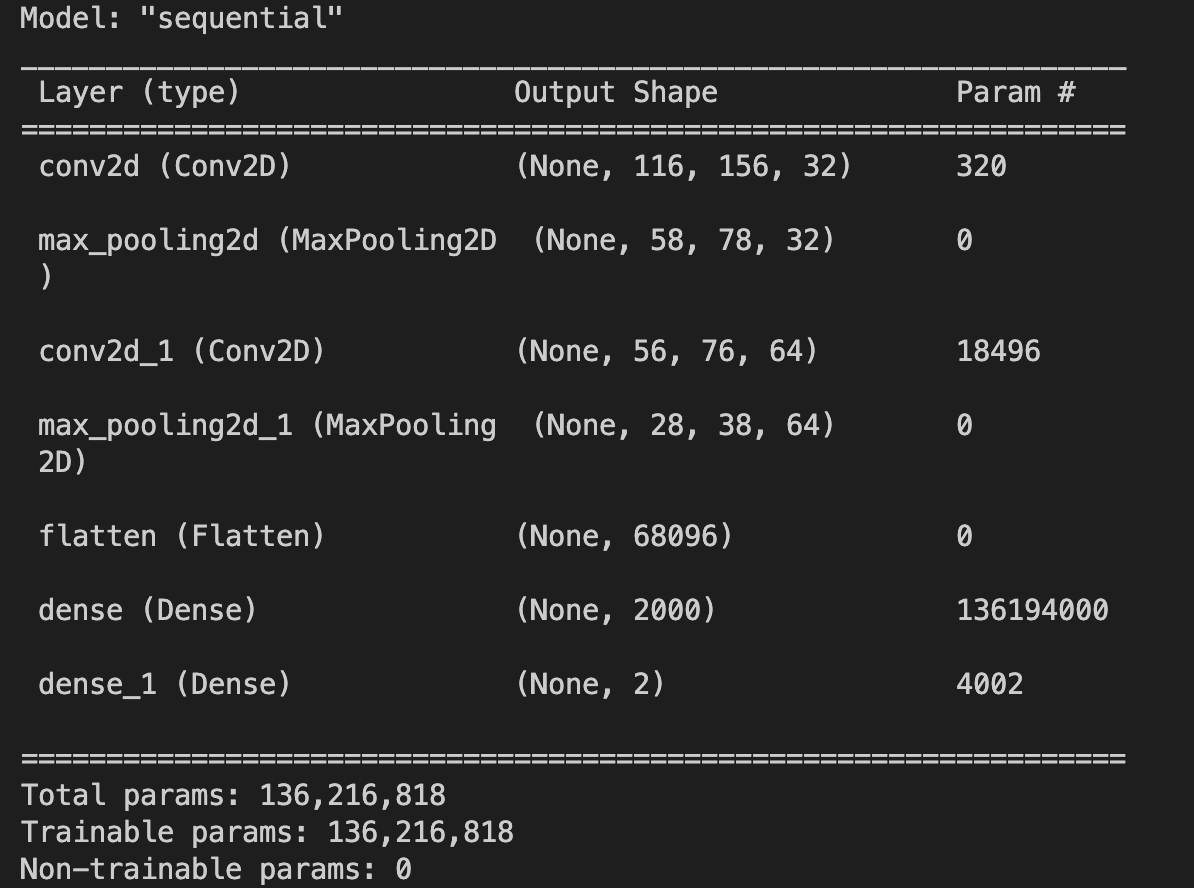
\includegraphics[width=0.6\linewidth]{figures/tensorflow_open_hand_fist_arch.png}
    \caption{Architecture of Keras Open Hand/Fist Classifier}
    \label{fig:tensorflow_open_hand_fist_arch}
\end{figure}

\begin{figure}[h]
    \centering
    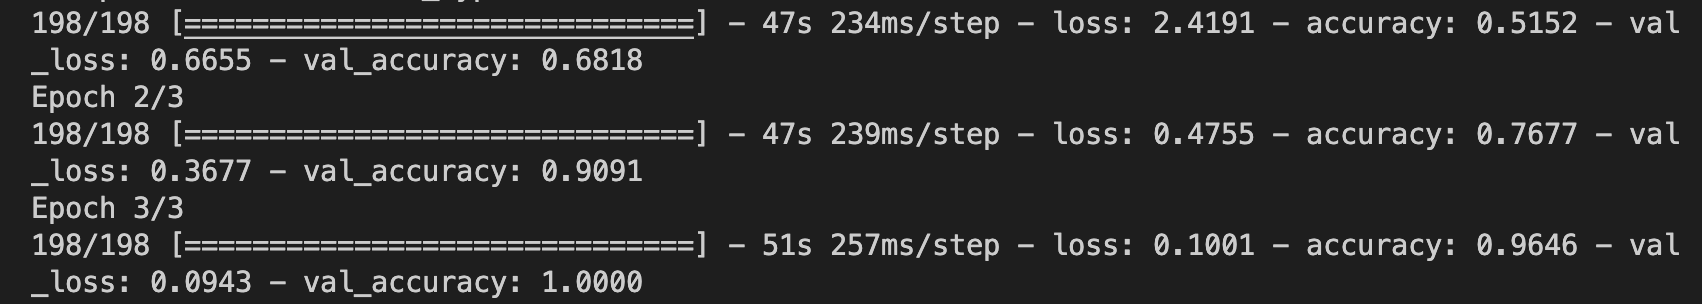
\includegraphics[width=0.7\linewidth]{figures/tensorflow_open_hand_fist_accuracy.png}
    \caption{Accuracy and loss of Keras Open Hand/Fist Classifier}
    \label{fig:tensorflow_open_hand_fist_accuracy}
\end{figure}

\begin{figure}[h]
    \centering
    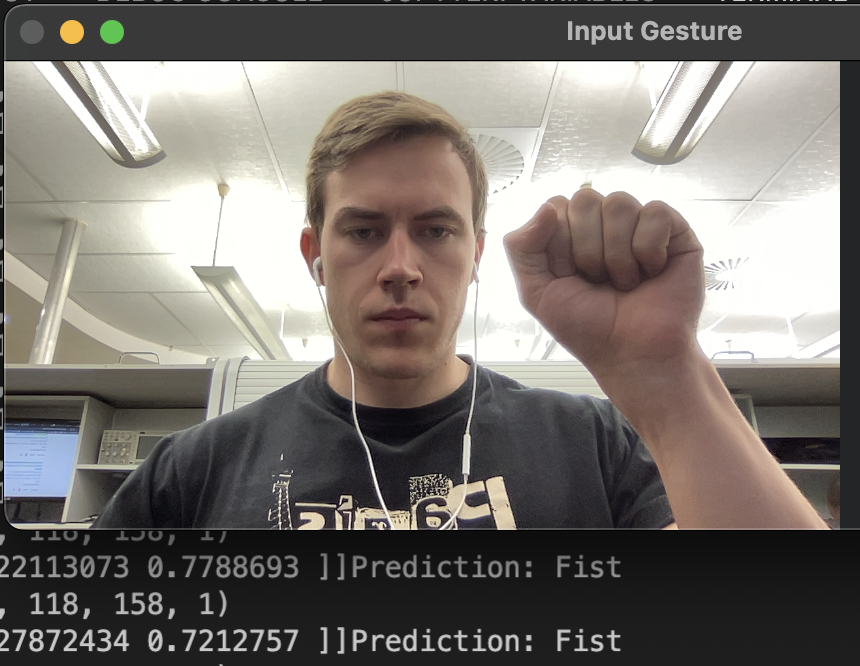
\includegraphics[width=0.6\linewidth]{figures/tensorflow_open_hand_fist_prediction1.png}
    \caption{Prediction of Keras Open Hand/Fist Classifier}
    \label{fig:tensorflow_open_hand_fist_prediction1}
\end{figure}

\begin{figure}[h]
    \centering
    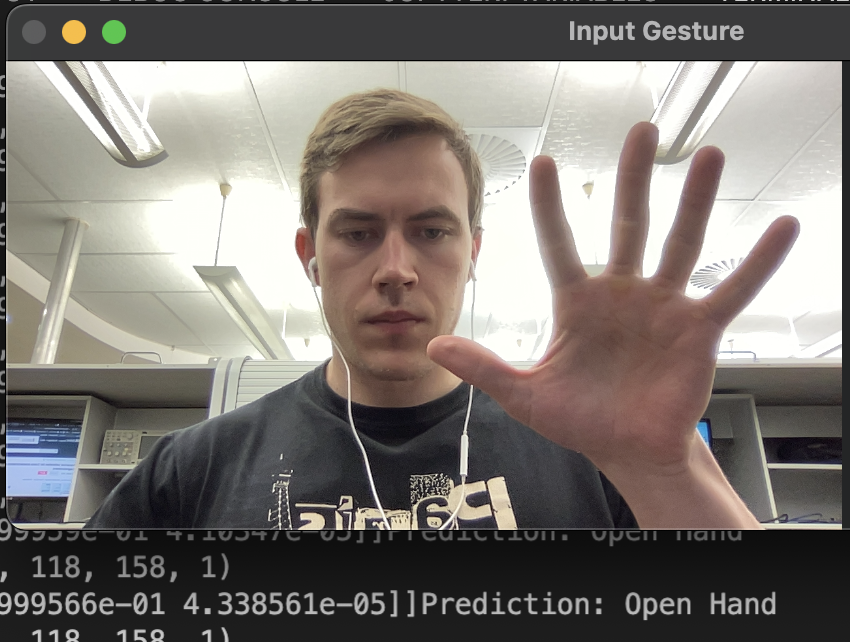
\includegraphics[width=0.6\linewidth]{figures/tensorflow_open_hand_fist_prediction2.png}
    \caption{Prediction of Keras Open Hand/Fist Classifier}
    \label{fig:tensorflow_open_hand_fist_prediction2}
\end{figure}

Much of the day was spent attempting to extend the result of the open hand/fist classifier to multiple gestures, however although an accuracy of 100\% could be attained on the training data, only about 80\% could be achieved on the testing data. This shows possible overfitting to the training data and a lack of training data overall in order to get the network to generalize the hand gesture shapes. Data augmentation was performed by flipping all the data across the vertical axis and essentially doubling the amount of training data. At the time of writing, the training process using this data was still underway.

What is of note is that the input to the network after edge detection currently is as seen in \FigRef{fig:NN_segmented_edge_detected}. A lot of background information is still retained in this image and may be confusing the network or allocating learning capability to classifying the background when it is useless. To this end, further segmentation was performed using the HSV and Ycbcr color spaces with masking this time around in order to more efficiently segment skin from background imagery. The results are visible in \FigRef{fig:hsv_segmentation_fast} and \FigRef{fig:ycbcr_segmentation_fast} and it is clear that the Ycbcr color space segmentation is still superior. 


\begin{figure}[h]
    \centering
    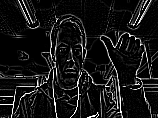
\includegraphics[width=0.6\linewidth]{figures/NN_segmented_edge_detected.png}
    \caption{Current input to network after segmentation}
    \label{fig:NN_segmented_edge_detected}
\end{figure}


\begin{figure}[h]
    \centering
    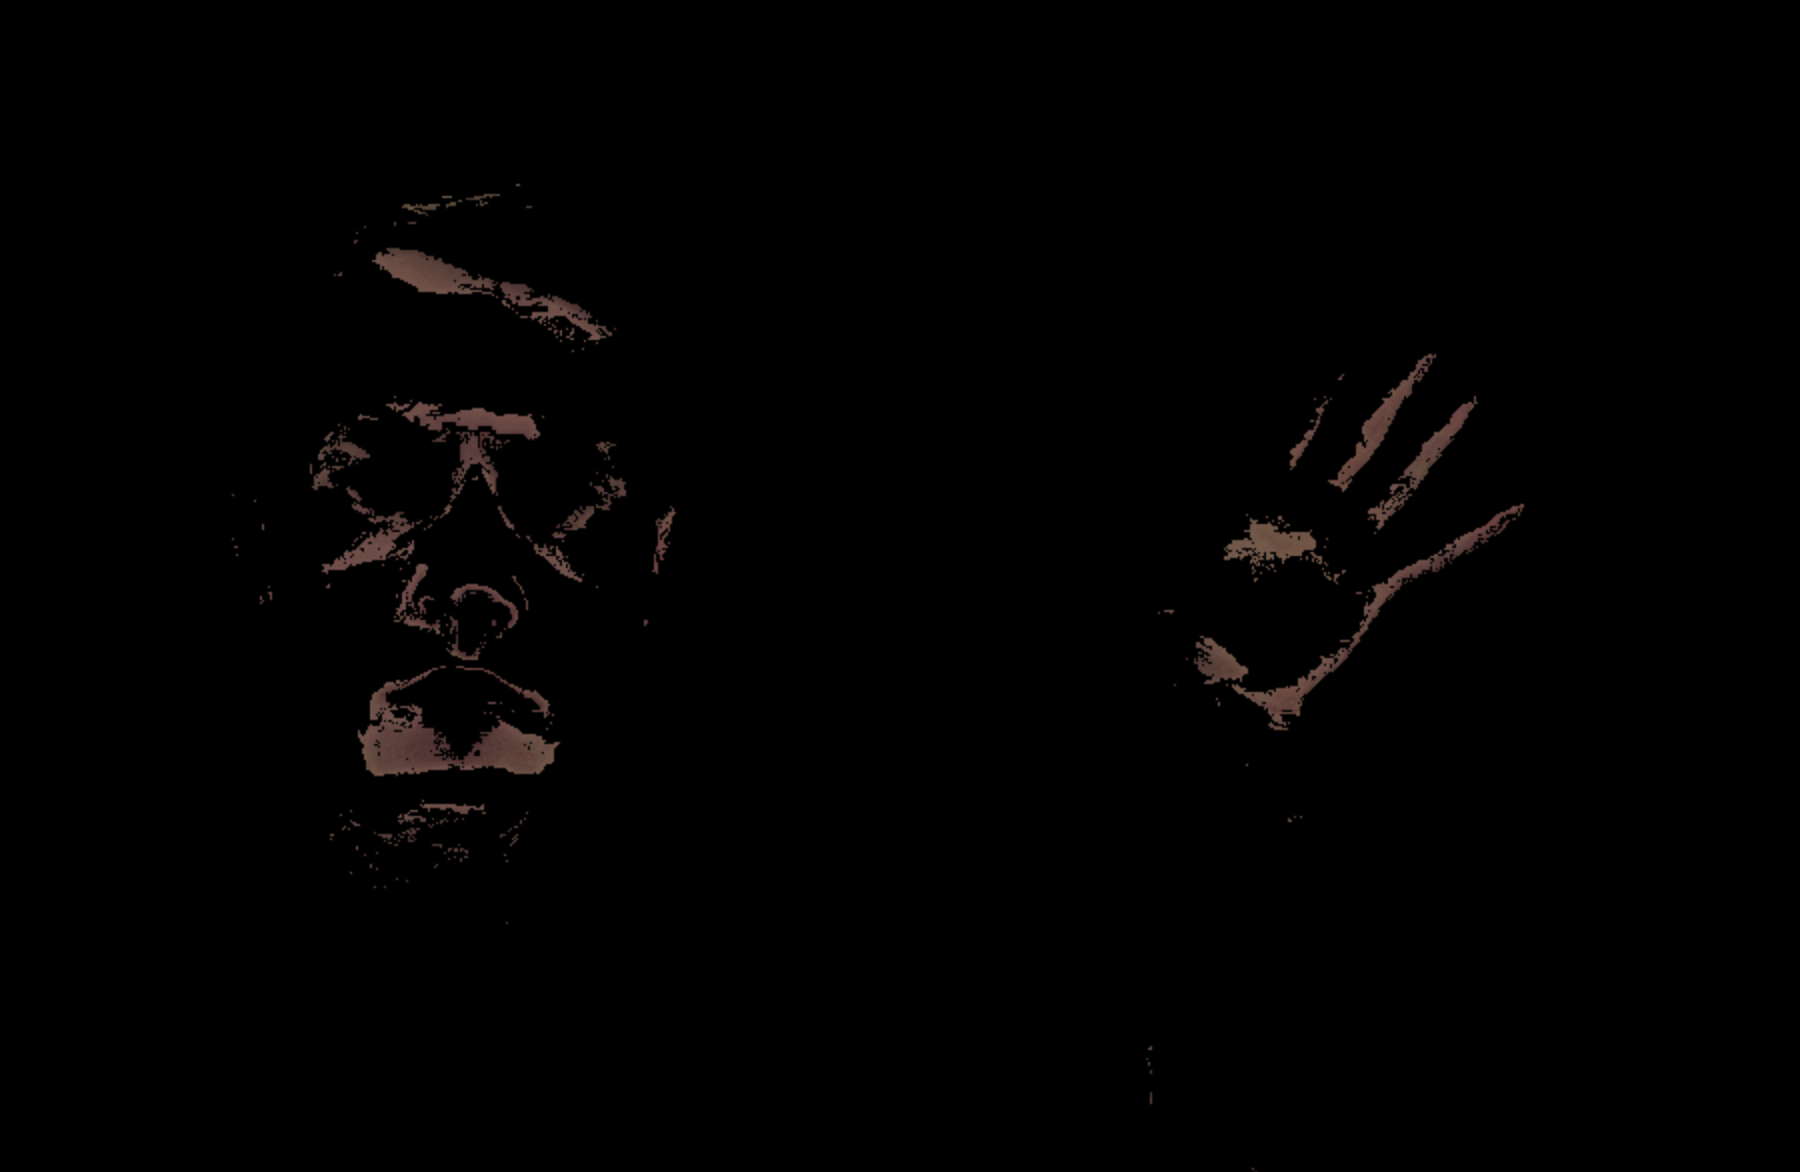
\includegraphics[width=0.6\linewidth]{figures/hsv_segmentation_fast.png}
    \caption{Segmentation using masking and the HSV color space}
    \label{fig:hsv_segmentation_fast}
\end{figure}

\begin{figure}[h]
    \centering
    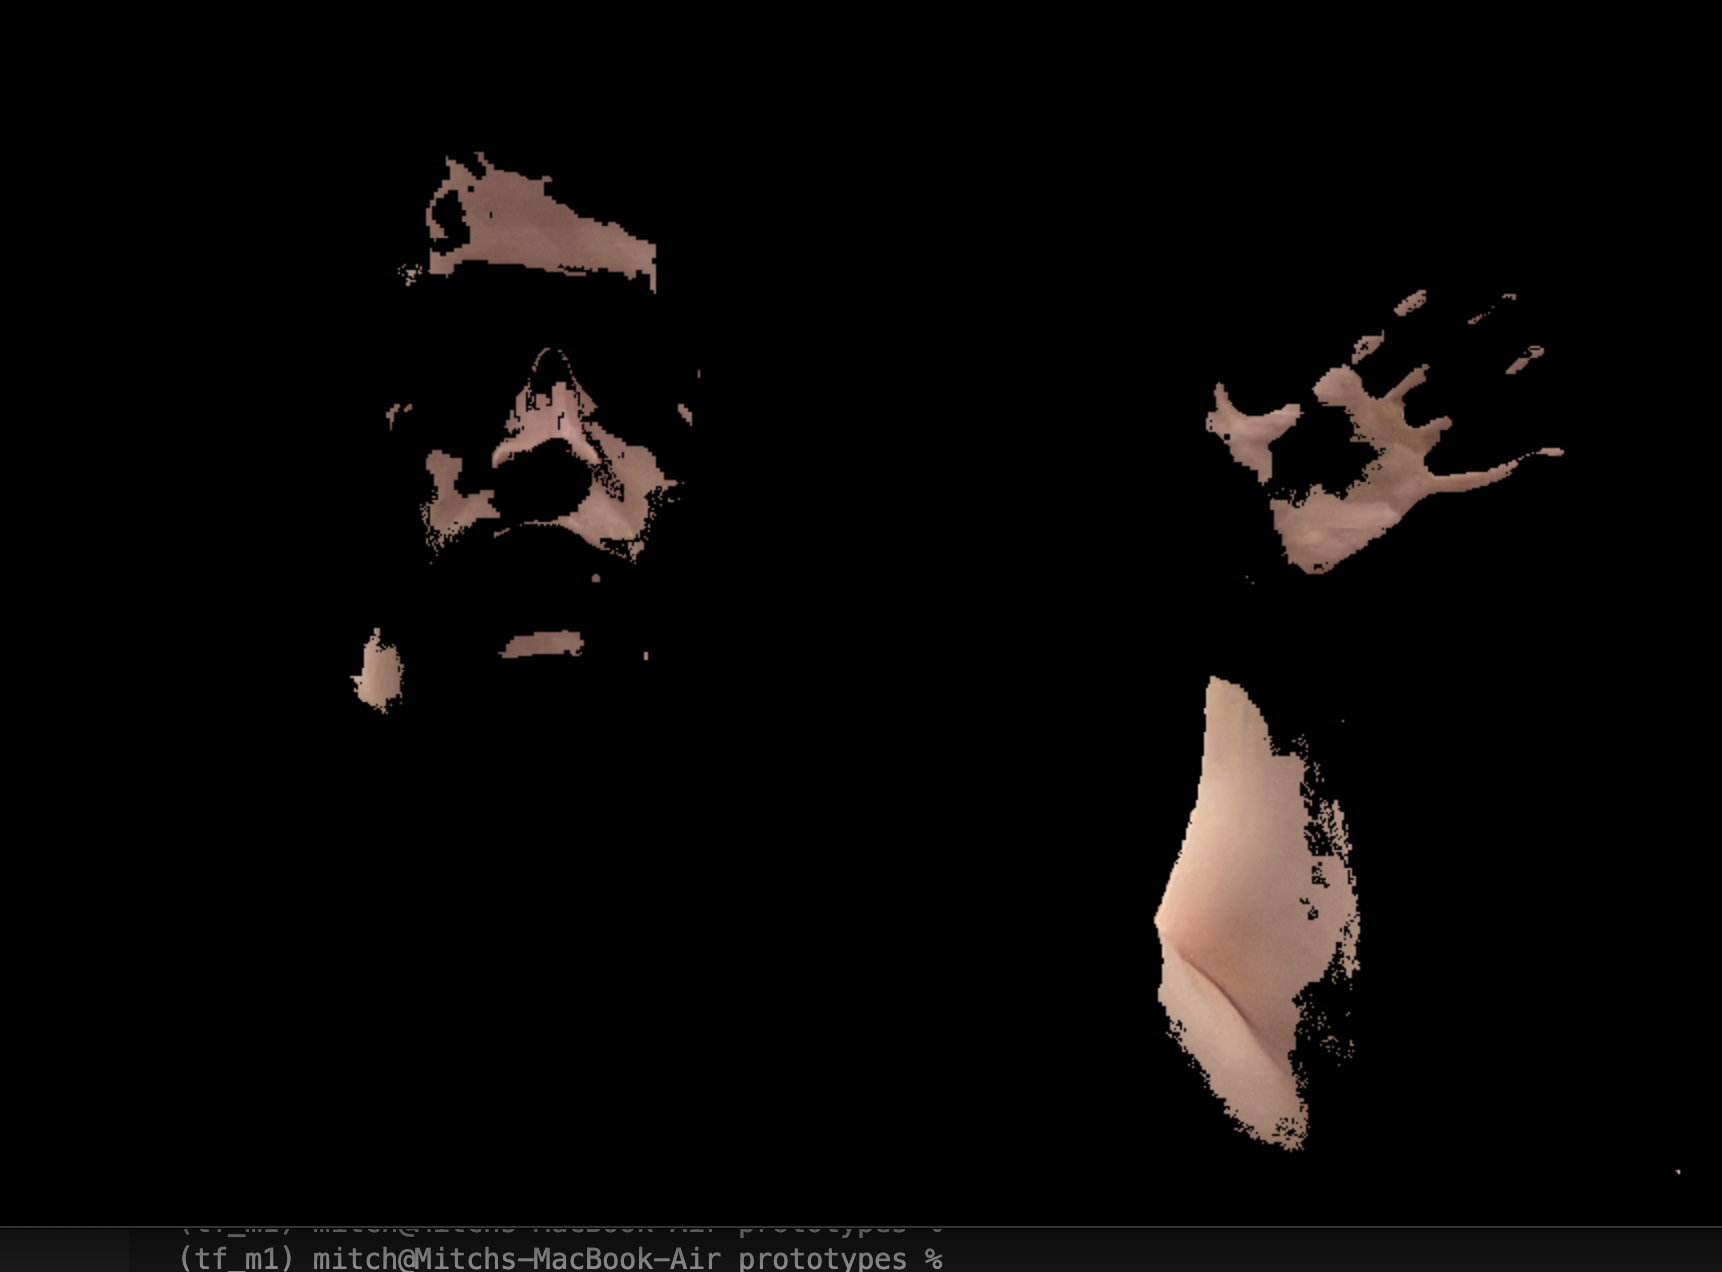
\includegraphics[width=0.6\linewidth]{figures/ycbcr_segmentation_fast.png}
    \caption{Segmentation using masking and the Ycbcr color space}
    \label{fig:ycbcr_segmentation_fast}
\end{figure}

This segmenting will thus be integrated into the preprocessing stage of the network and is hypothesized to increase training accuracy and the system's performance.

\section[2022/08/15]{Monday, 15 August 2022}

\subsection{Discussion of current gesture recognition system inadequacies}

The use of Keras to train and build prototype gesture recognition systems has met with success. As shown above, these prototypes can tell the difference between an open and closed hand with good accuracy on both a training and testing dataset however real-world performance suffers when the system is provided with novel input from a webcam. The system is not yet good enough to accurately classify gestures in new and novel positions. A number of optimizations can thus be pursued to increase the accuracy of the system. These are increasing the amount of training data, increasing the size of the network and implementing a hand detector system to reduce the amount of input given to the system. \\

On this last suggestion, the current input to the system is the segmented skin region parts of an image as seen in \FigRef{fig:network_skin_segmented_input} and although this considerably simplifies what the system has to learn, it still contains the parts of the image corresponding to the user's face and it is hypothesized that this extra input is confusing the network or rather wasting its resources trying to classify parts of the face that aren't relative to the hand gesture being displayed. Thus the construction of a hand detector that can recognize the pixels of the image that belong to the hand and segment only them from the background could be a way to reduce the input complexity to the system and improve gesture detection accuracy. \\

Training the network with input data that only contains images of hands in various gestures without faces present in the images is also a possible way of increasing the accuracy of the system and will be attempted as well. Thus the next tasks to complete in order to increase the accuracy of the gesture recognition system are as follows.

\begin{itemize}
    \item Re-train gesture recognition network using input images without faces present
    \item Increase amount of training data provided to system
    \item Increase size of the network used for classification
    \item Construct a hand detector to further segment the hand from the remainder of the input image
  \end{itemize}

\begin{figure}[h]
    \centering
    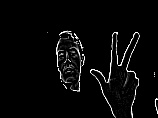
\includegraphics[width=0.3\linewidth]{figures/network_skin_segmented_input.png}
    \caption{Current segmented input to the system}
    \label{fig:network_skin_segmented_input}
\end{figure}

While attempting to re-train the network with images devoid of faces it was discovered that the system is sensitive to lighting changes and the edge detection filter outputs close-to-junk data if the lighting conditions change drastically. The lighting changes between two sets of input data are shown in \FigRef{fig:error_segmentation_2} and the junk data result of the edge detection filter with a different lighting condition to what it was initially setup with is shown in \FigRef{fig:error_segmentation}. Thus for further experimentation, sensitivity to lighting conditions will have to be taken into account in order to achieve consistent output. The importance of cleaning data before it is fed into a machine learning system is thus clearly demonstrated by this problem and will be rectified in future.

\begin{figure}[h]
    \centering
    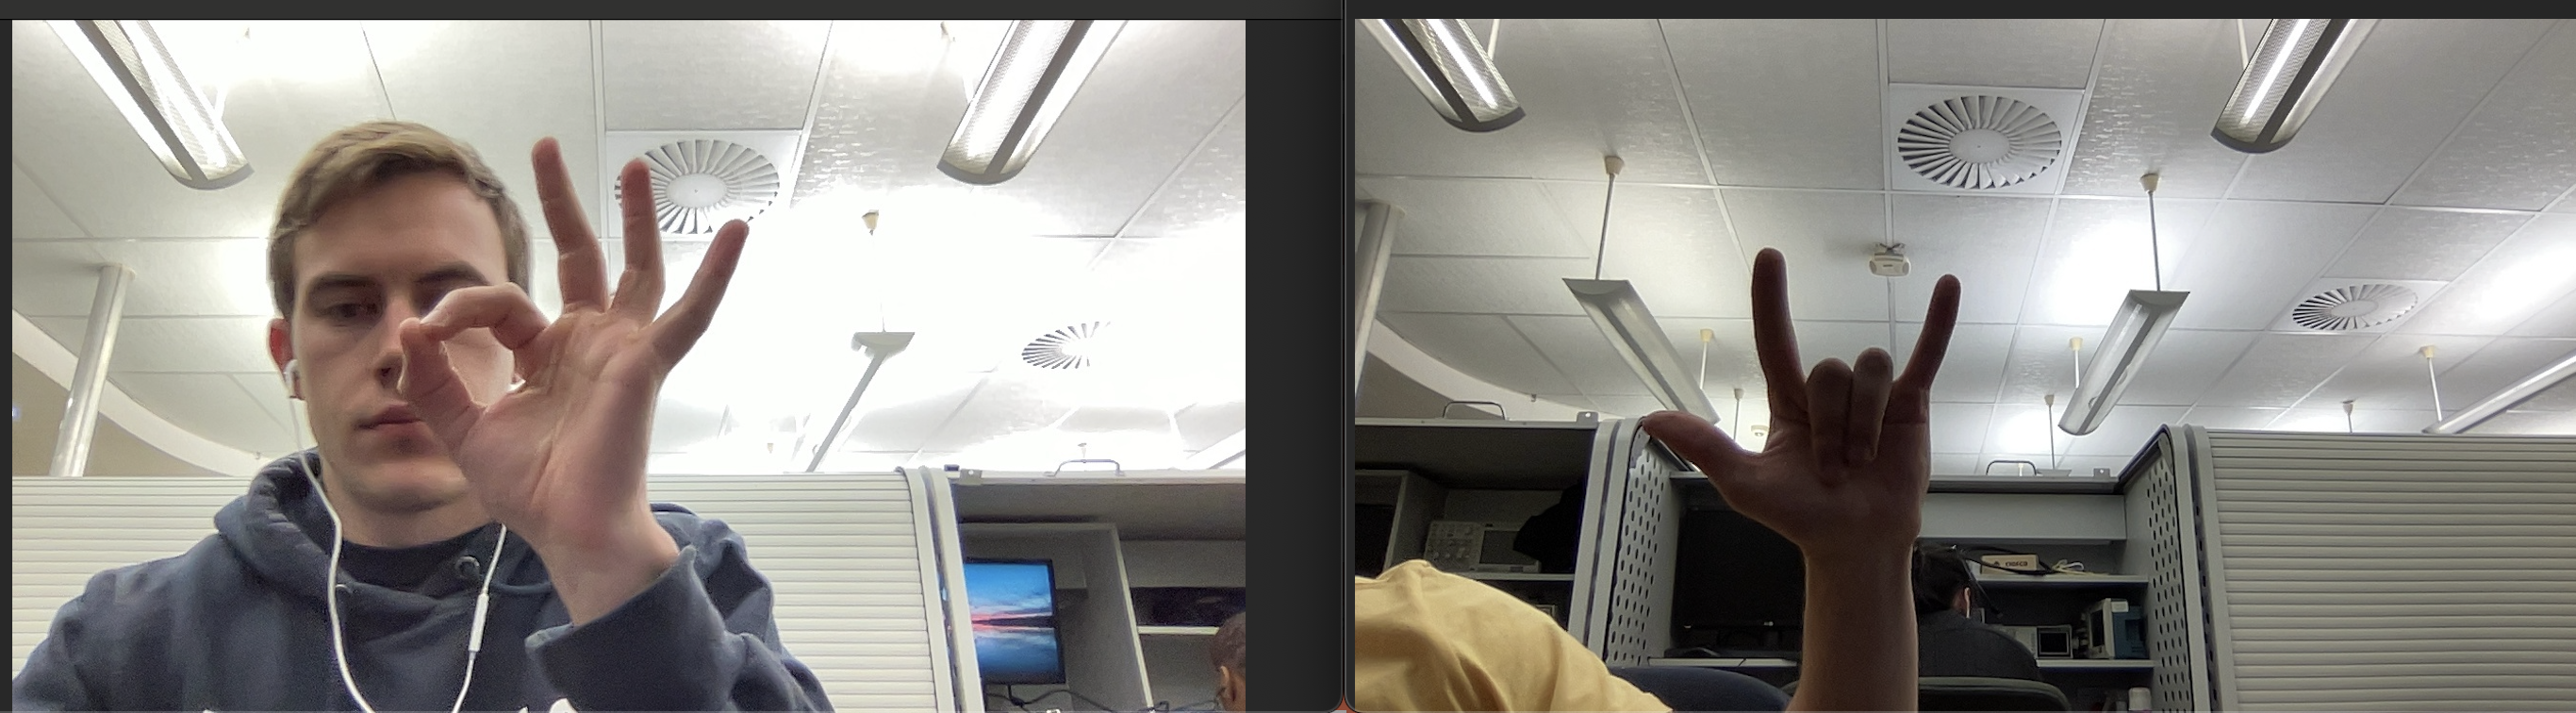
\includegraphics[width=1.0\linewidth]{figures/error_segmentation_2.png}
    \caption{Different lighting inputs to the gesture recognition system}
    \label{fig:error_segmentation_2}
\end{figure}

\begin{figure}[h]
    \centering
    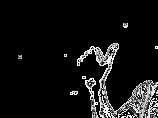
\includegraphics[width=0.6\linewidth]{figures/error_segmentation.png}
    \caption{Current segmented input to the system}
    \label{fig:error_segmentation}
\end{figure}

\section[2022/08/16]{Tuesday, 16 August 2022}

\subsection{Construction of updated prototype implementation}

The aim of today's work session is to construct up-to-date prototypes of the system.

Previously, an OpenGL movement API was developed that could take in a value between 0 and 1 for each an x, y and z coordinate value and normalize this to the width and height of the screen. This normalized value would then be the destination coordinates for a cube rendered in OpenGL. Because OpenGL only has rotations and translations a small API was developed that could take in these world coordinates and transform them to the corresponding translation and rotation commands that OpenGL could render and appear to move the cube to the correct coordinates. This was done by finding the delta between the current and desired coordinates and translating the OpenGL cube by these delta amounts as well as adding extra translations in the x and y directions when the cube was translated in a z-direction in order to keep it in place but correctly "grow" or "shrink" the cube from the user's perspective. This movement API was used extensively in the following prototypes.

The first prototype is built using OpenGL and Mediapipe and it is a pinky-tracking cube movement system. The location of the pinky finger in a webcam input is found using Mediapipe and the OpenGL cube movement API designed from first principles accepts a coordinate as input and then snaps the cube to the location of the pinky finger. In this way, rudimentary tracking can be achieved. The result of the prototype can be seen in \FigRef{fig:OpenGL_mediapipe_prototype_pinky_tracker}.

\begin{figure}[h]
    \centering
    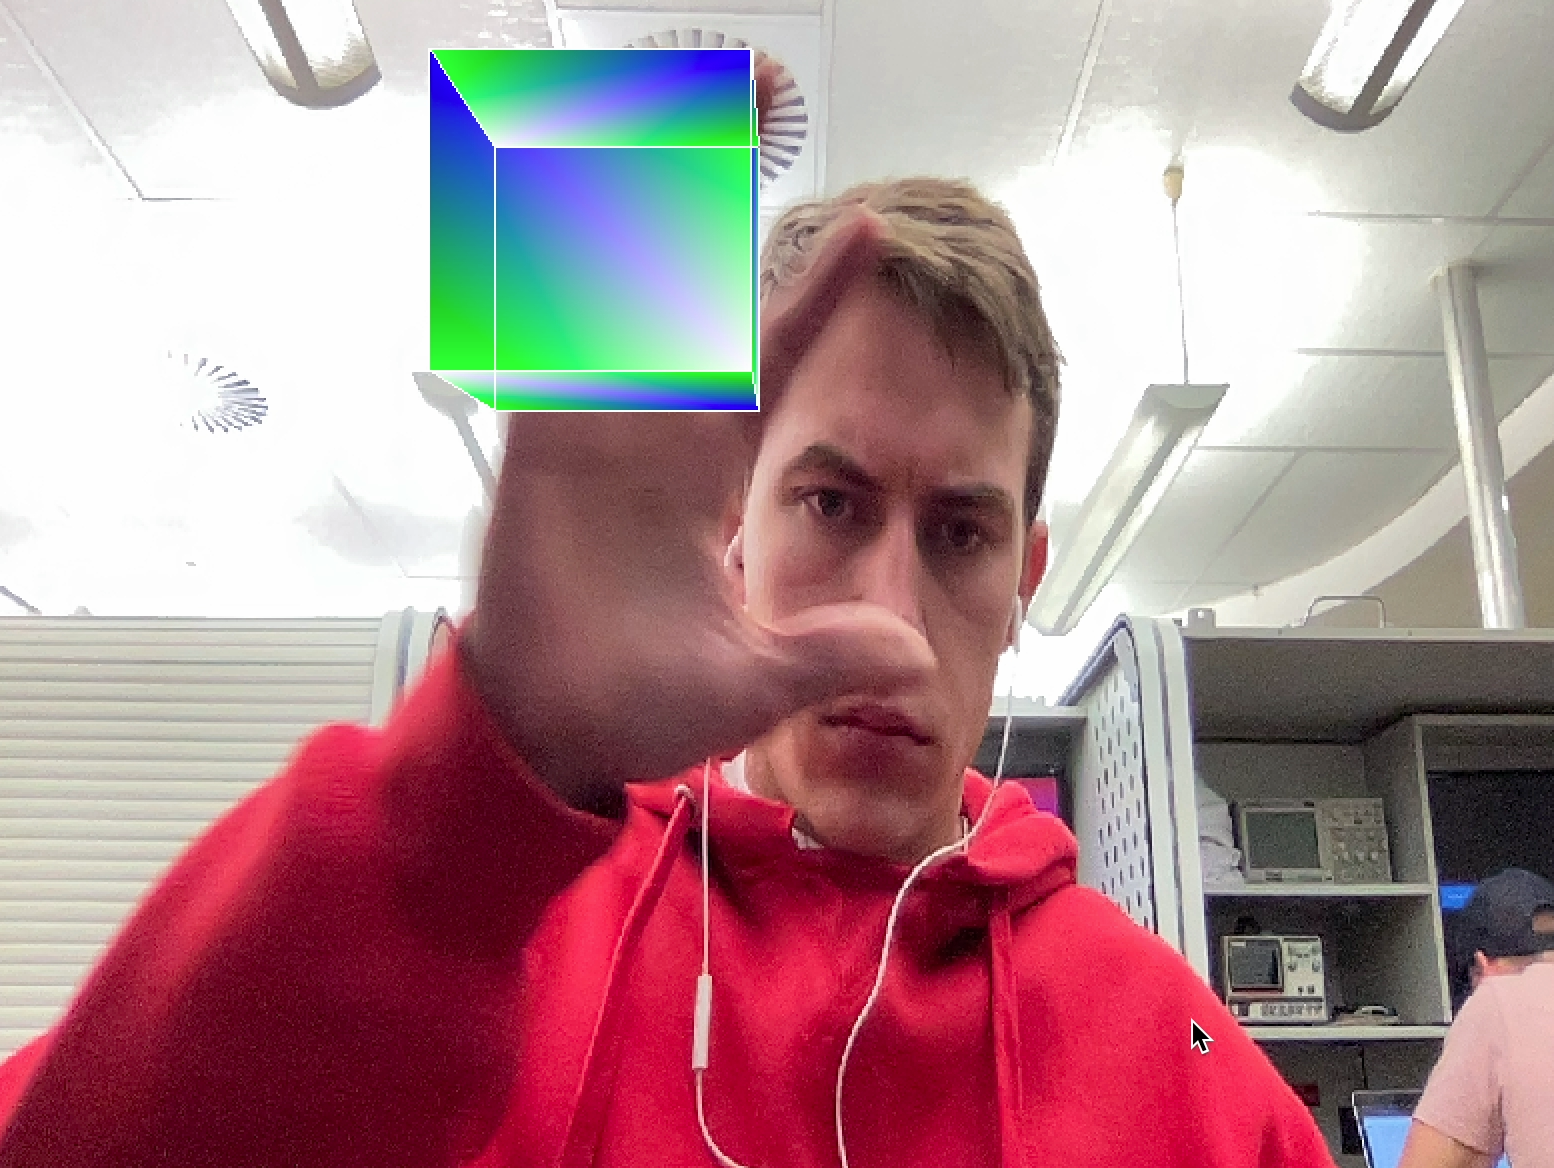
\includegraphics[width=0.6\linewidth]{figures/OpenGL_mediapipe_prototype_pinky_tracker.png}
    \caption{OpenGL and Mediapipe Pinky Tracker Prototype}
    \label{fig:OpenGL_mediapipe_prototype_pinky_tracker}
\end{figure}

The second prototype is built using the same OpenGL movement API developed but this time with a small Tensorflow convolutional neural network for detecting whether input webcam images contain a closed fist or open hand. The operation of this system is visible in \FigRef{fig:OpenGL_tensorflow_fist_open_hand}. Based on the detected gesture the cube is either snapped to the left or right of the screen. The accuracy of the model is 1.0 on the training data and nearly the same on the test dataset however it performs with middling accuracy on real-live webcam input. This is once again hypothesized to be due to the changing lighting conditions when a hand is adjusted slightly so that it reflects more of the ceiling lights - this is affecting the segmentation algorithm which discriminates a hand based on skin colour and illuminance and so optimizing the network to be robust to changing lighting conditions is necessary in order to get it to accurately recognize gestures.

\begin{figure}[h]
    \centering
    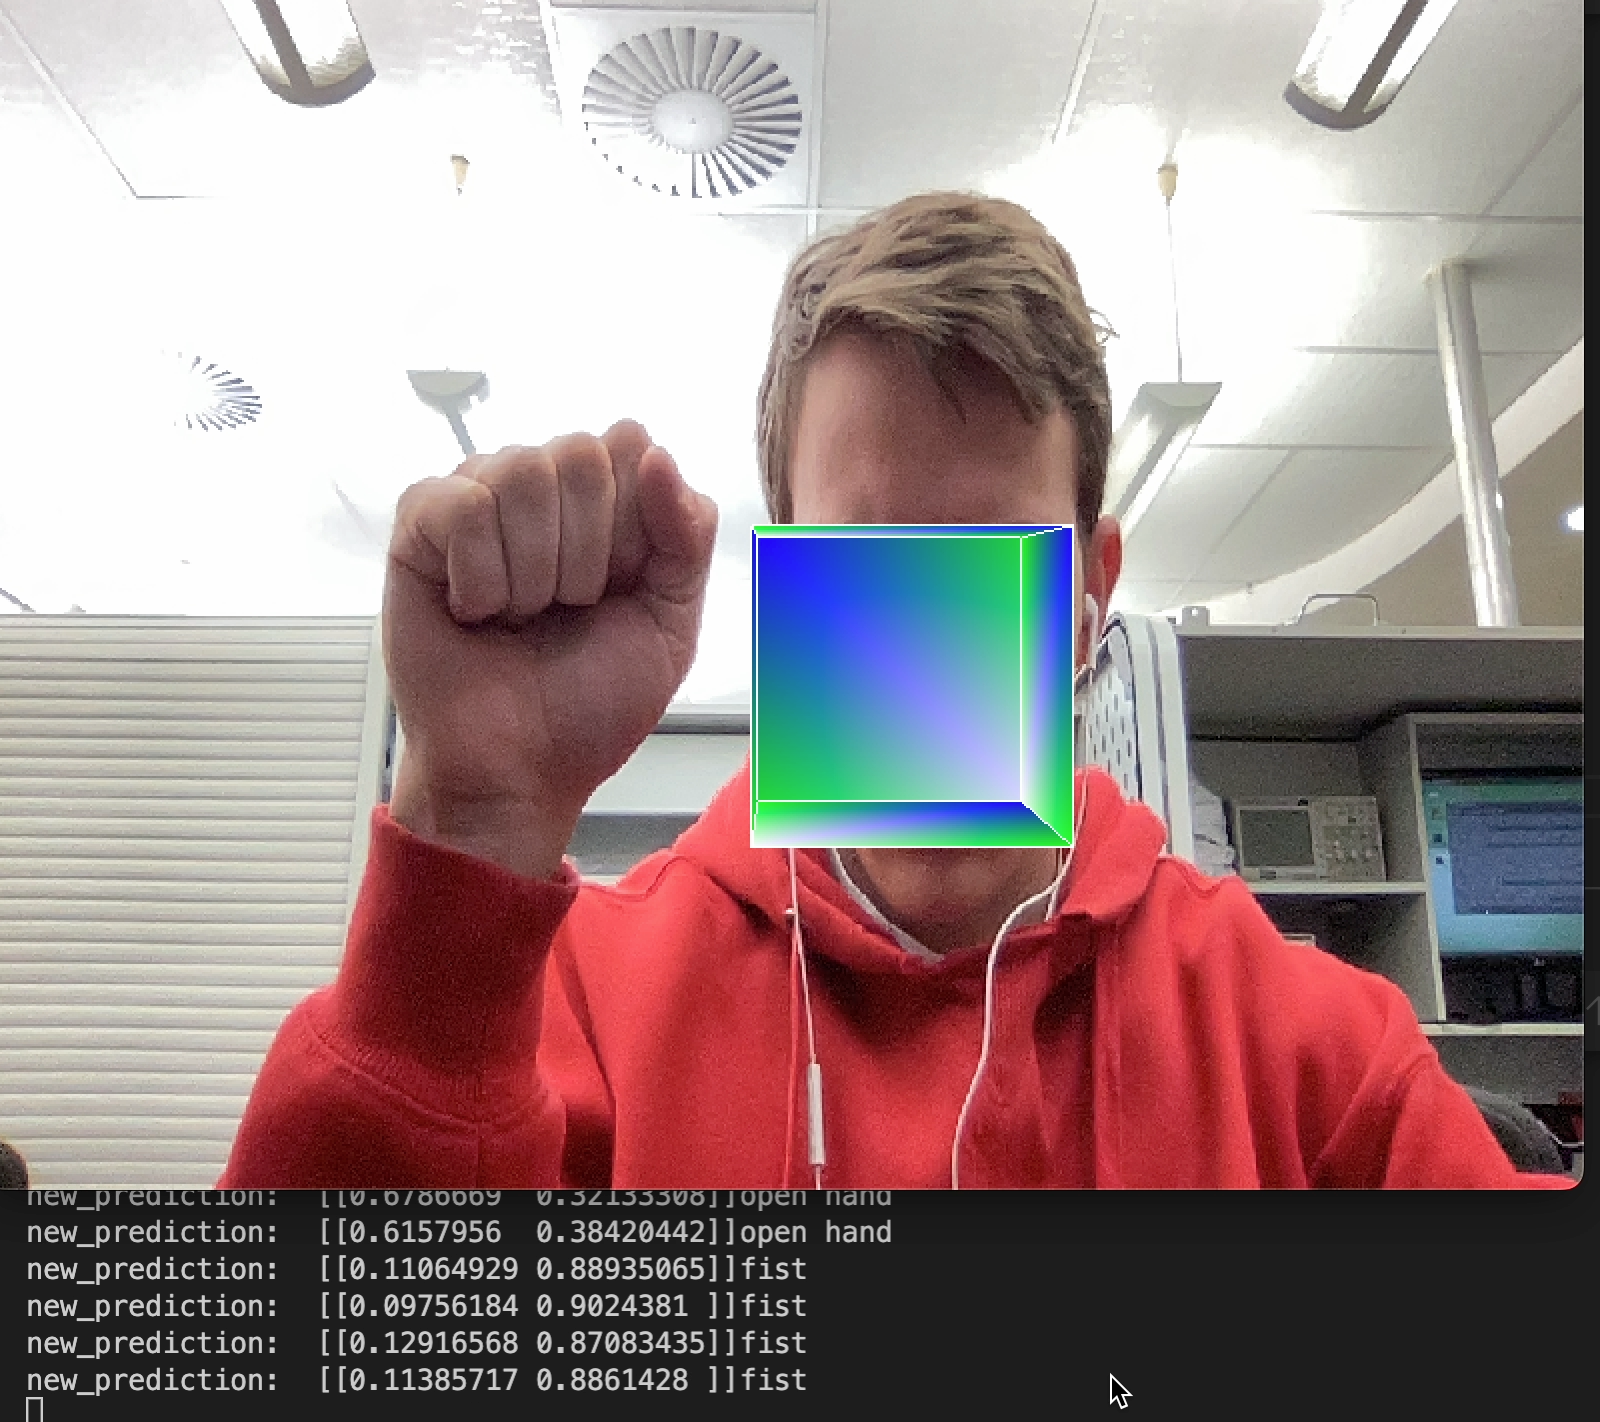
\includegraphics[width=0.6\linewidth]{figures/OpenGL_tensorflow_fist_open_hand.png}
    \caption{OpenGL and Tensorflow Fist/Open Hand Prototype}
    \label{fig:OpenGL_tensorflow_fist_open_hand}
\end{figure}

The final prototype constructed uses the same OpenGL movement API and the Kinect sensor to perform object collision avoidance between the virtual object and real-world environment. The x and z keys are pressed on the keyboard and alternatively move the cube to two different locations on the screen - which have corresponding x and y coordinates. At the same time, the Kinect sensor receives depth data for the entire width and height of the screen and this depth data is examined for a certain value in a range between 500 and 700, which is roughly a metre and a half from the camera. If there is a value in this range anywhere near the x and y coordinates that the cube is about to be moved to, the cube is prevented from moving there and an object "collision" is registered. The operation of the system is visible in \FigRef{fig:OpenGL_Kinect_collision_avoidance} and shows the user trying to move the cube back to the top left of the screen but the system preventing the action from taking place because the user is located there and is taking up the space there. This basic prototype shows that the Kinect depth data can be used to prevent object collisions between real and virtual objects with moderate speed and accuracy. Scaling up the object detection system and matching the OpenGL cube coordinates to those of the image is the next major hurdle.

\begin{figure}[h]
    \centering
    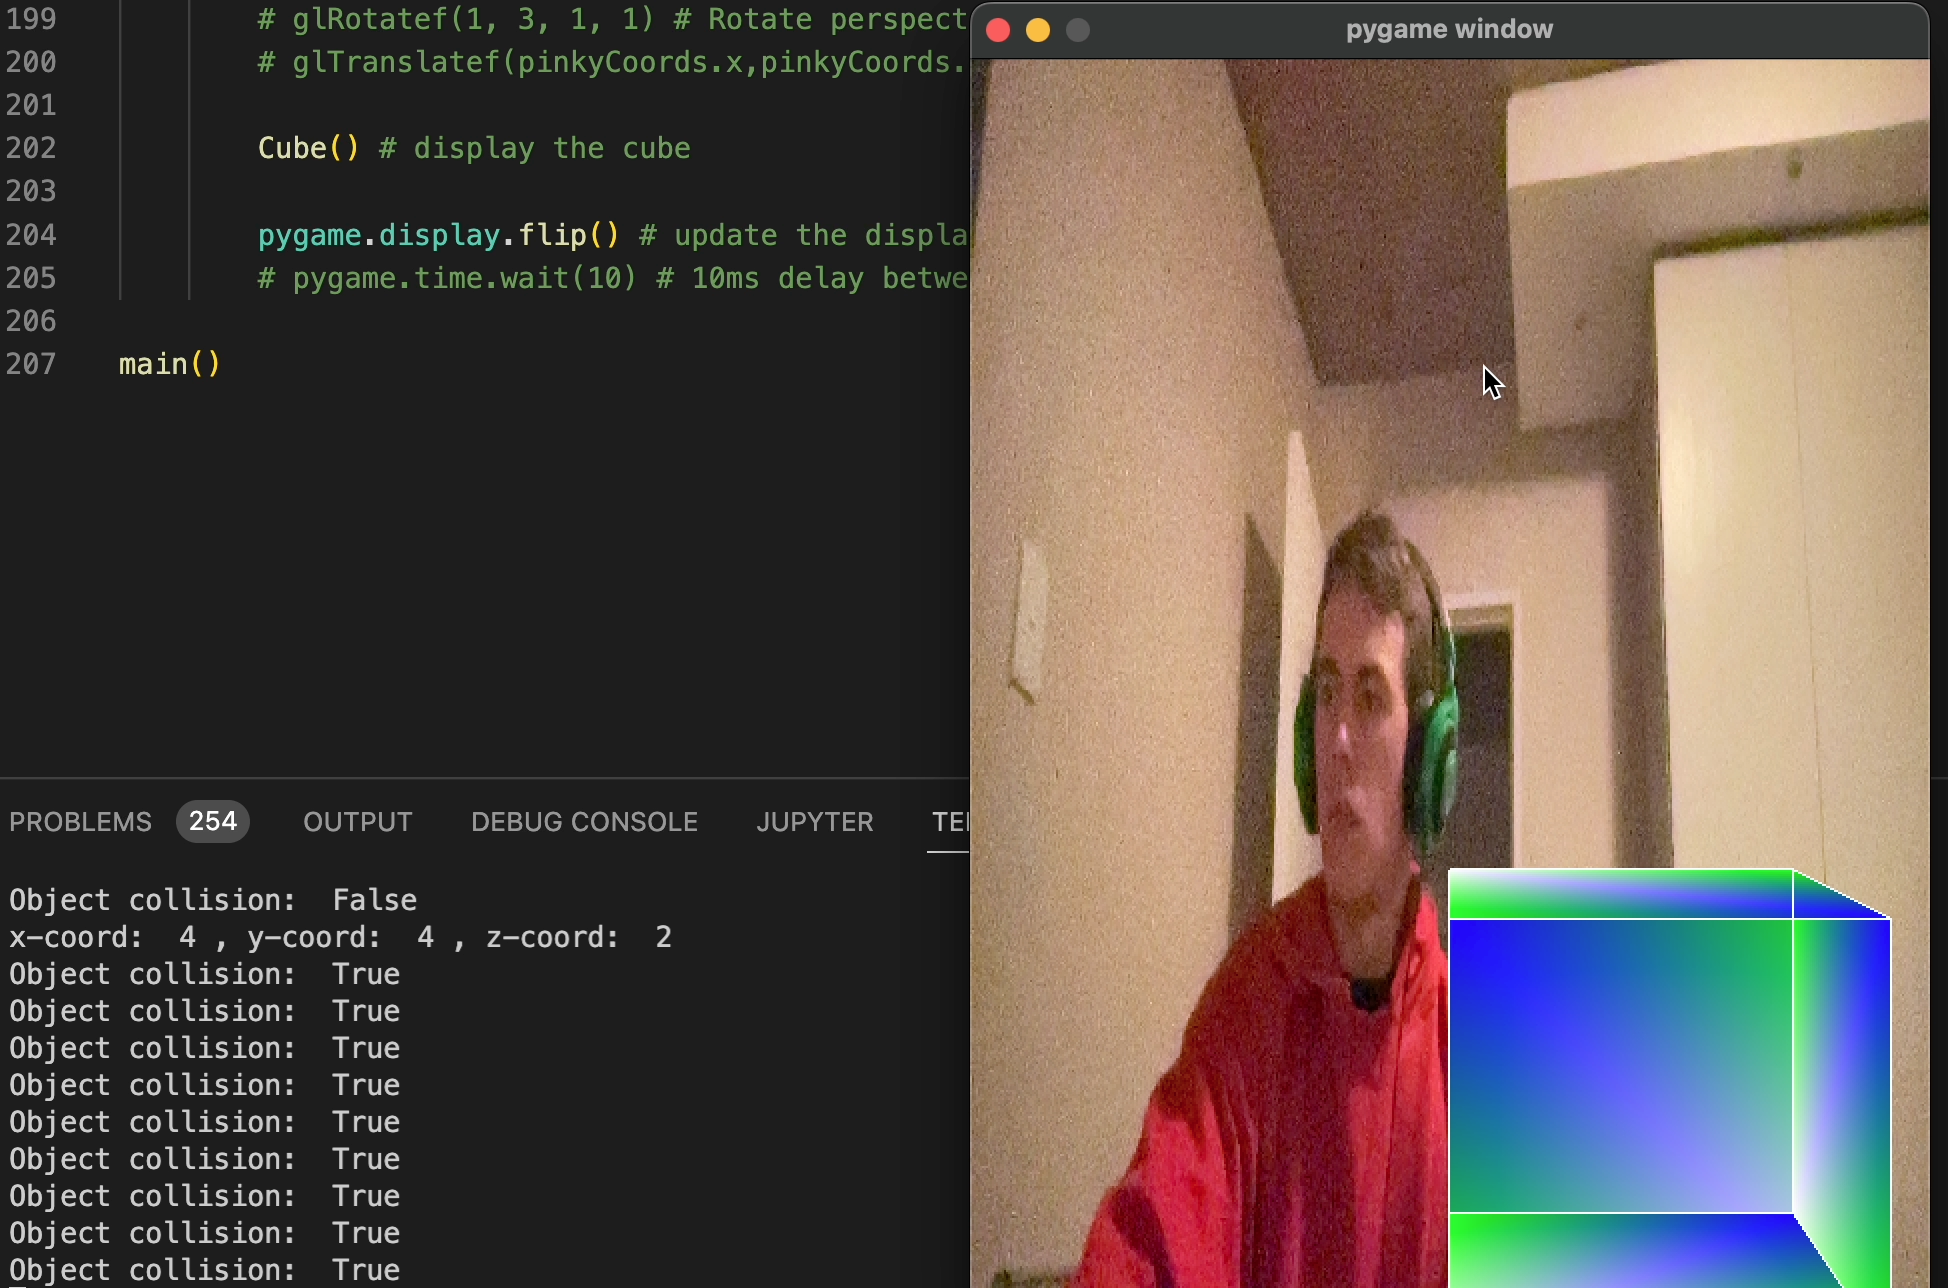
\includegraphics[width=0.9\linewidth]{figures/OpenGL_Kinect_collision_avoidance.png}
    \caption{OpenGL and Kinect Collision Avoidance Prototype}
    \label{fig:OpenGL_Kinect_collision_avoidance}
\end{figure}

Additionally, after attempting many methods, the exposure of the webcam used to generate training images and perform hand gesture inferences was set to a constant value using the Camera Controller application. The settings are visible in \FigRef{fig:camera_controller_exposure_settings} and are hypothesized to make training the hand gesture recognition system much more reliable as segmentation based on the Ycbcr colorspace will be consistent and not changed by arbitrary lighting conditions.

\begin{figure}[h]
    \centering
    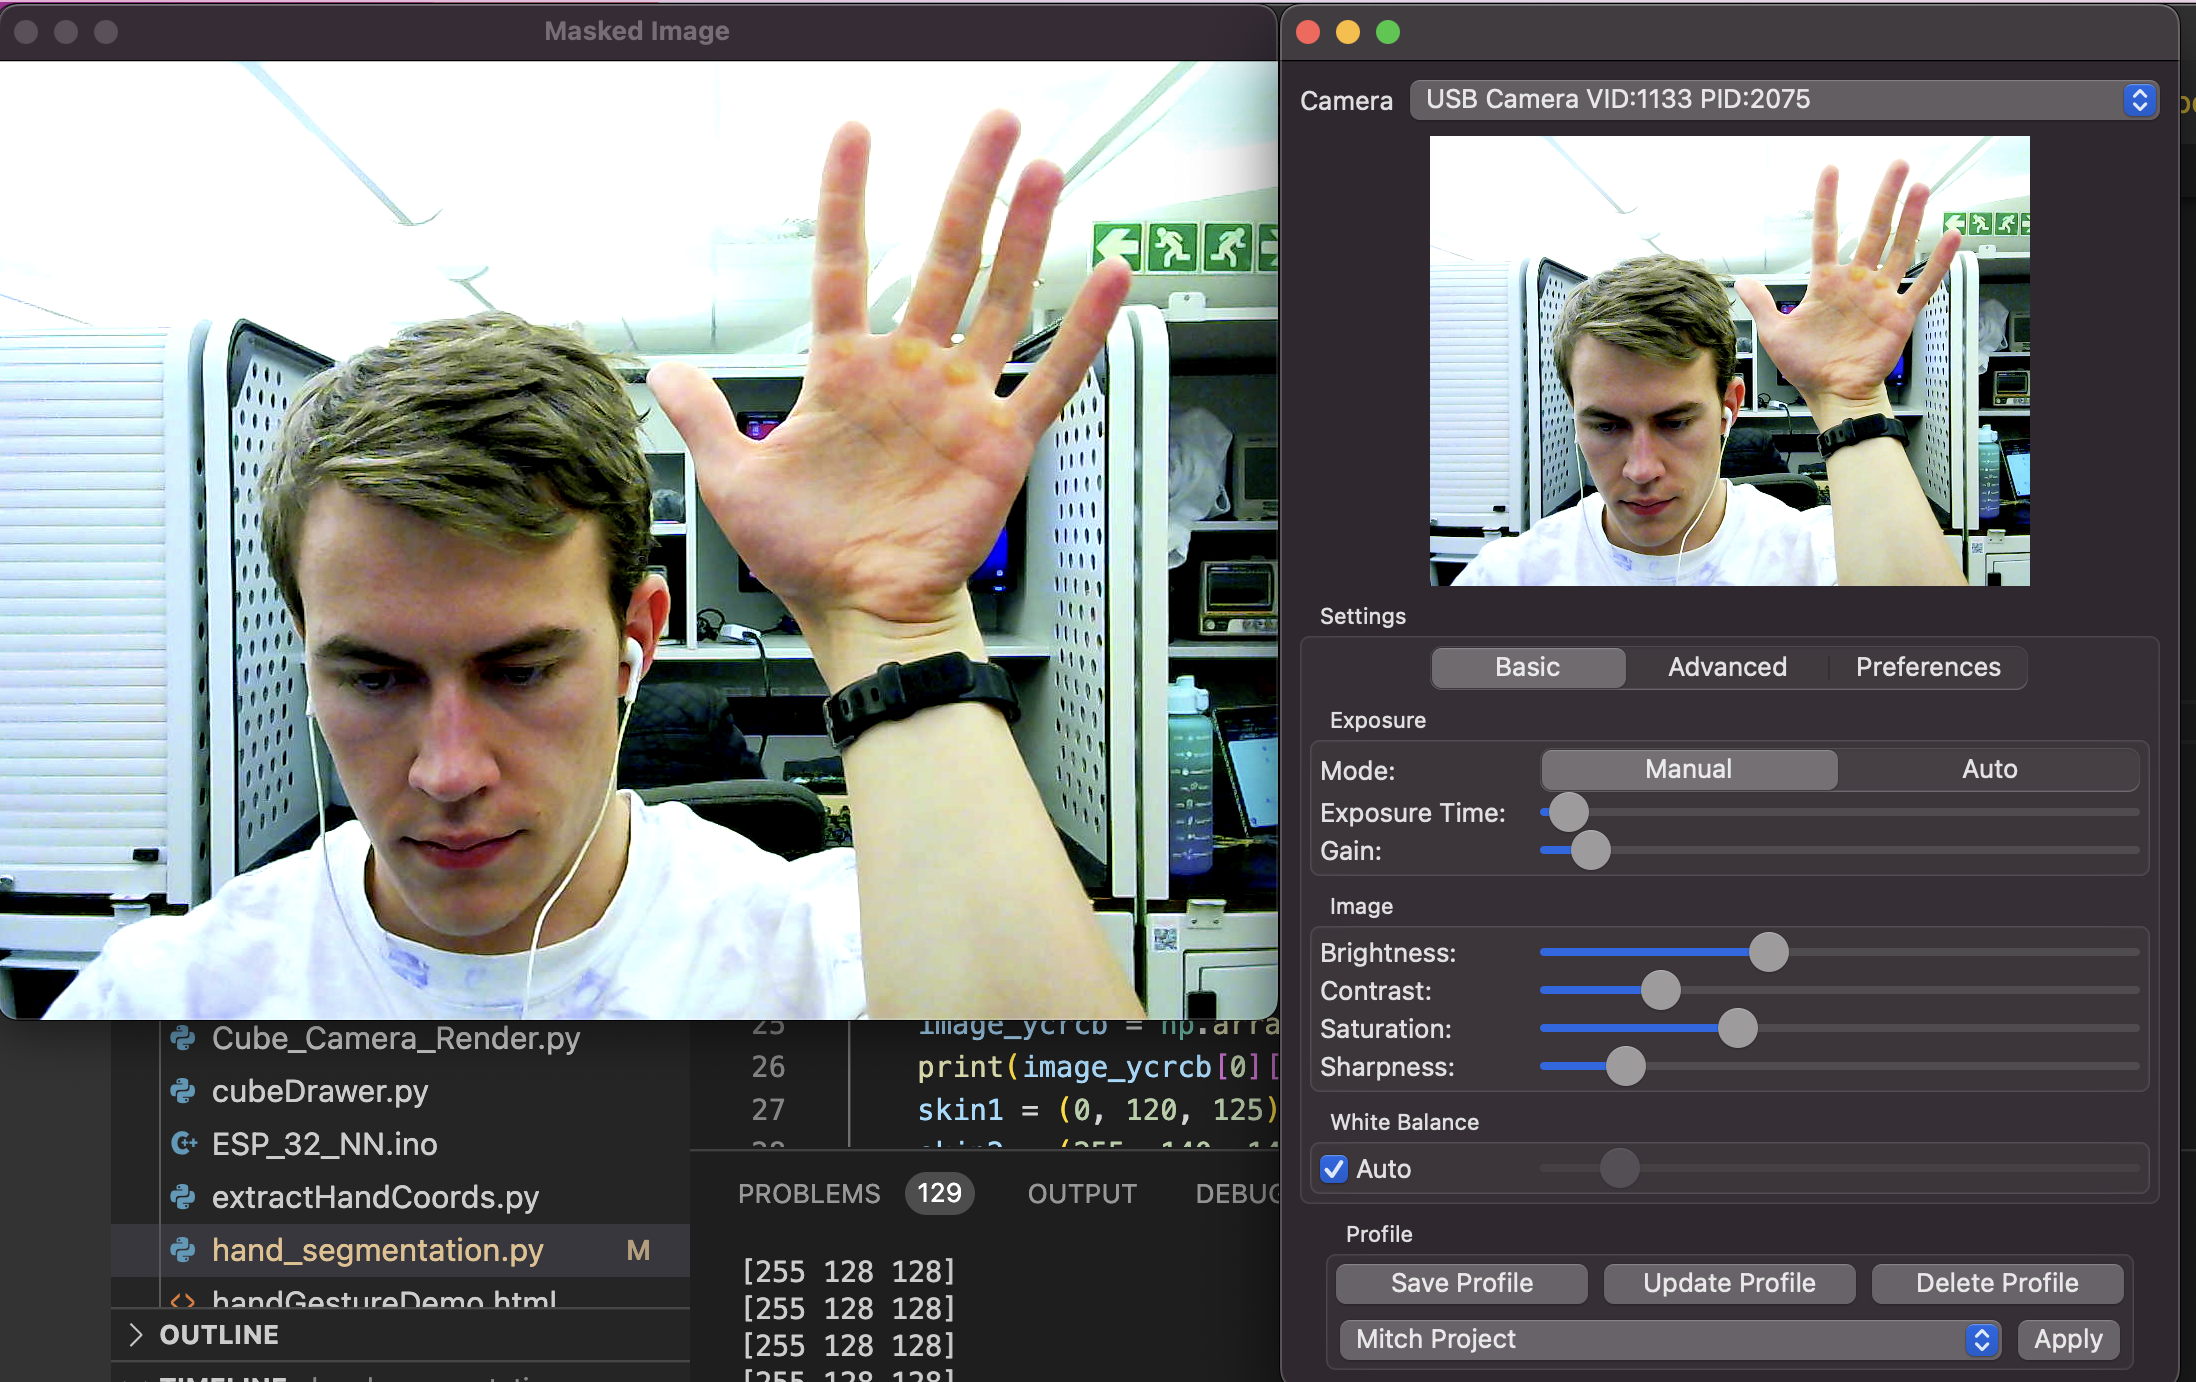
\includegraphics[width=0.9\linewidth]{figures/camera_controller_exposure_settings.png}
    \caption{Camera controller settings}
    \label{fig:camera_controller_exposure_settings}
\end{figure}

\section[2022/08/18]{Thursday, 18 August 2022}

\subsection{Gesture recognition system changes and demonstration planning}

The final objective of the system is to perform real-time gesture control of a virtual object in augmented reality. This will be demonstrated in a physical demonstration and thus the placement of the various cameras will affect the final performance of the system and how the training and testing will take place. The proposed hardware setup is illustrated in \FigRef{fig:proposed_camera_setup} and shows how the Kinect camera will be placed to the side of the table and the the webcam positioned above the desk. This is so that the virtual object can be interacted with on the tabletop and the depth data for the table and distance from the camera calculated. Furthermore, it simplifies the hand recognition/segmentation by using a top-down view which will not have the user's face in frame but rather just their hand and part of their arm. This gave rise to potential simplifer solutions for identifying the location of the hand in the frame such as simple color segmenting and even a contour-based approach, which will speed up the development and implementation considerably. This top-down view is presented in \FigRef{fig:topdown_view}

\begin{figure}[h]
    \centering
    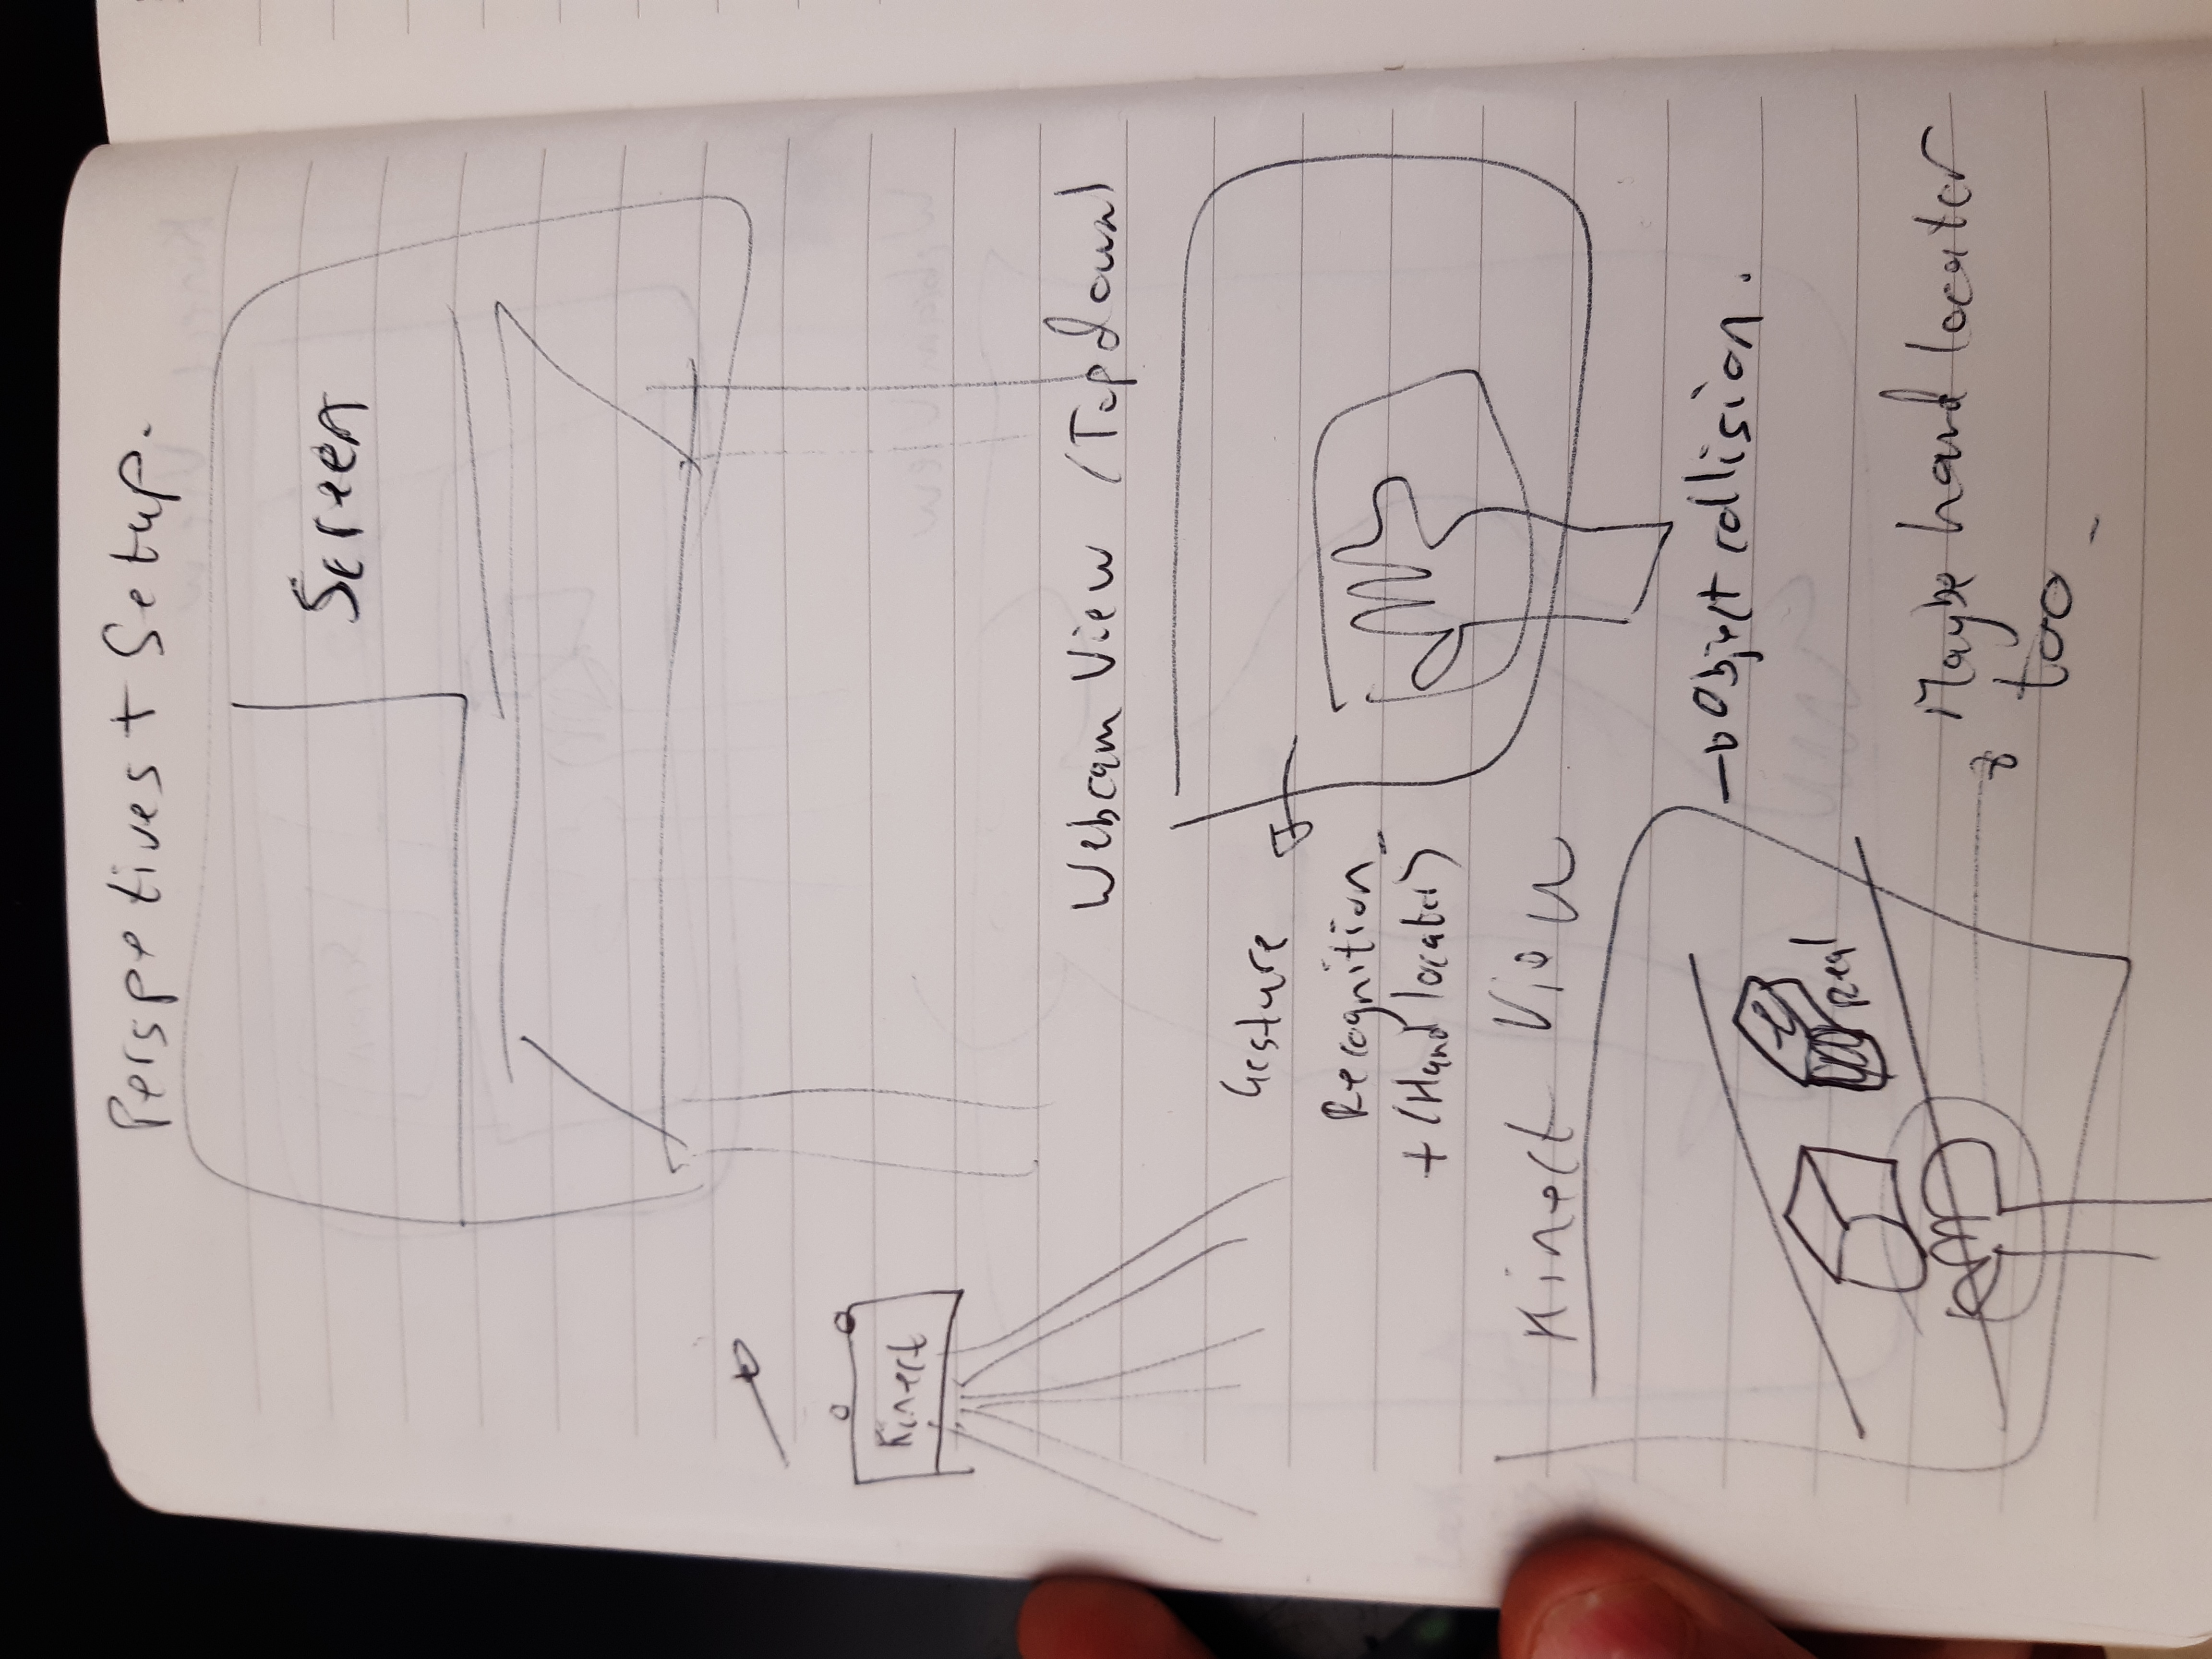
\includegraphics[width=0.7\linewidth]{figures/proposed_camera_setup.jpg}
    \caption{Proposed camera and hardware setup for demonstration}
    \label{fig:proposed_camera_setup}
\end{figure}

\begin{figure}[h]
    \centering
    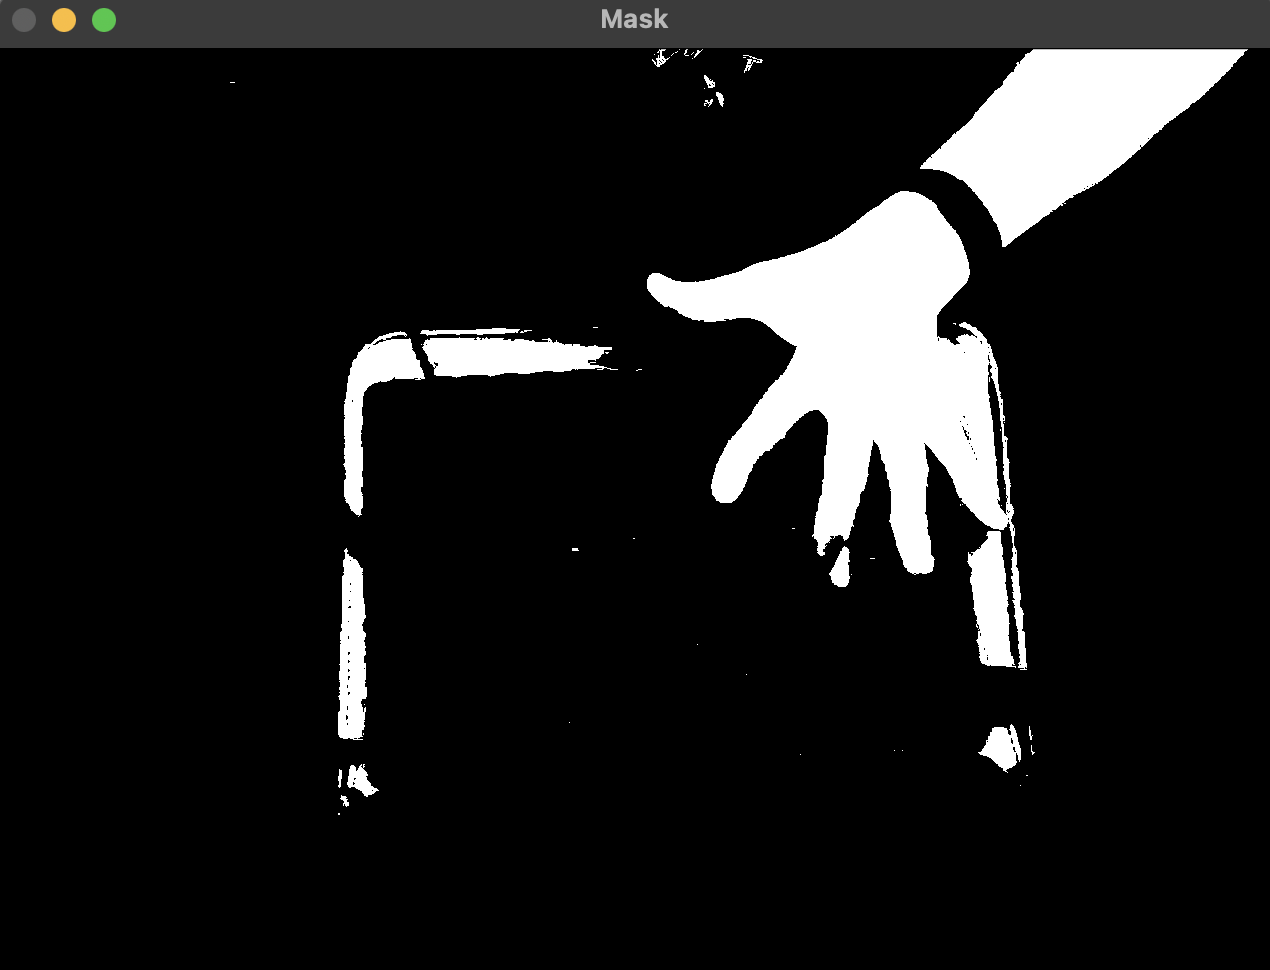
\includegraphics[width=0.7\linewidth]{figures/topdown_view.png}
    \caption{Proposed camera top-down view}
    \label{fig:topdown_view}
\end{figure}

\section[2022/08/19]{Friday, 19 August 2022}

\subsection{Hand locator}

The aim of this session is to build a hand detector system.

In order to do this a CNN will be used and trained on a collection of top-down pictures of hands present in the image. A tool for labelling these hands has been built using OpenCV and the images can be labelled by moving the rectangle over the hand using the keyboard and then saving the position of the box. The image is split into 22x17 = 374 individual regions which can either have a hand present in it or not. One of these regions is shown overlain on the hand in \FigRef{fig:hand_locator_tool}.

\begin{figure}[h]
    \centering
    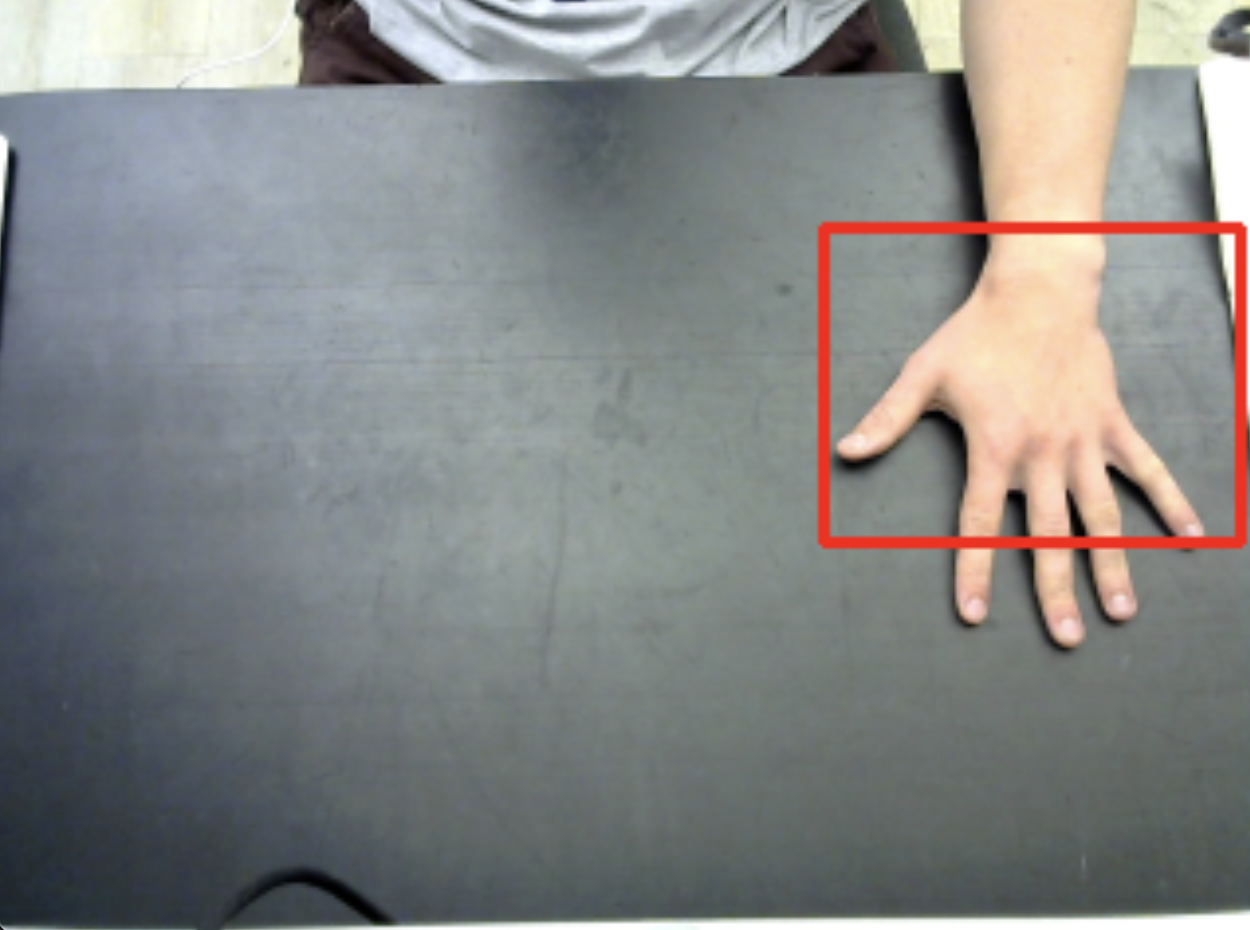
\includegraphics[width=0.7\linewidth]{figures/hand_locator_tool.png}
    \caption{Hand locator tool}
    \label{fig:hand_locator_tool}
\end{figure}

For all of the training images, the centre of the palm was determined by the user placing a rectangle over the hand in an interactive program and then extracting the image width and height coordinate from the centre of that rectangle. Delta values were then computed for all the candidate regions in the image based on their distance from the extracted palm coordinate. This is visible in the heatmap shown in \FigRef{fig:heatmap_hand_detector}.

\begin{figure}[h]
    \centering
    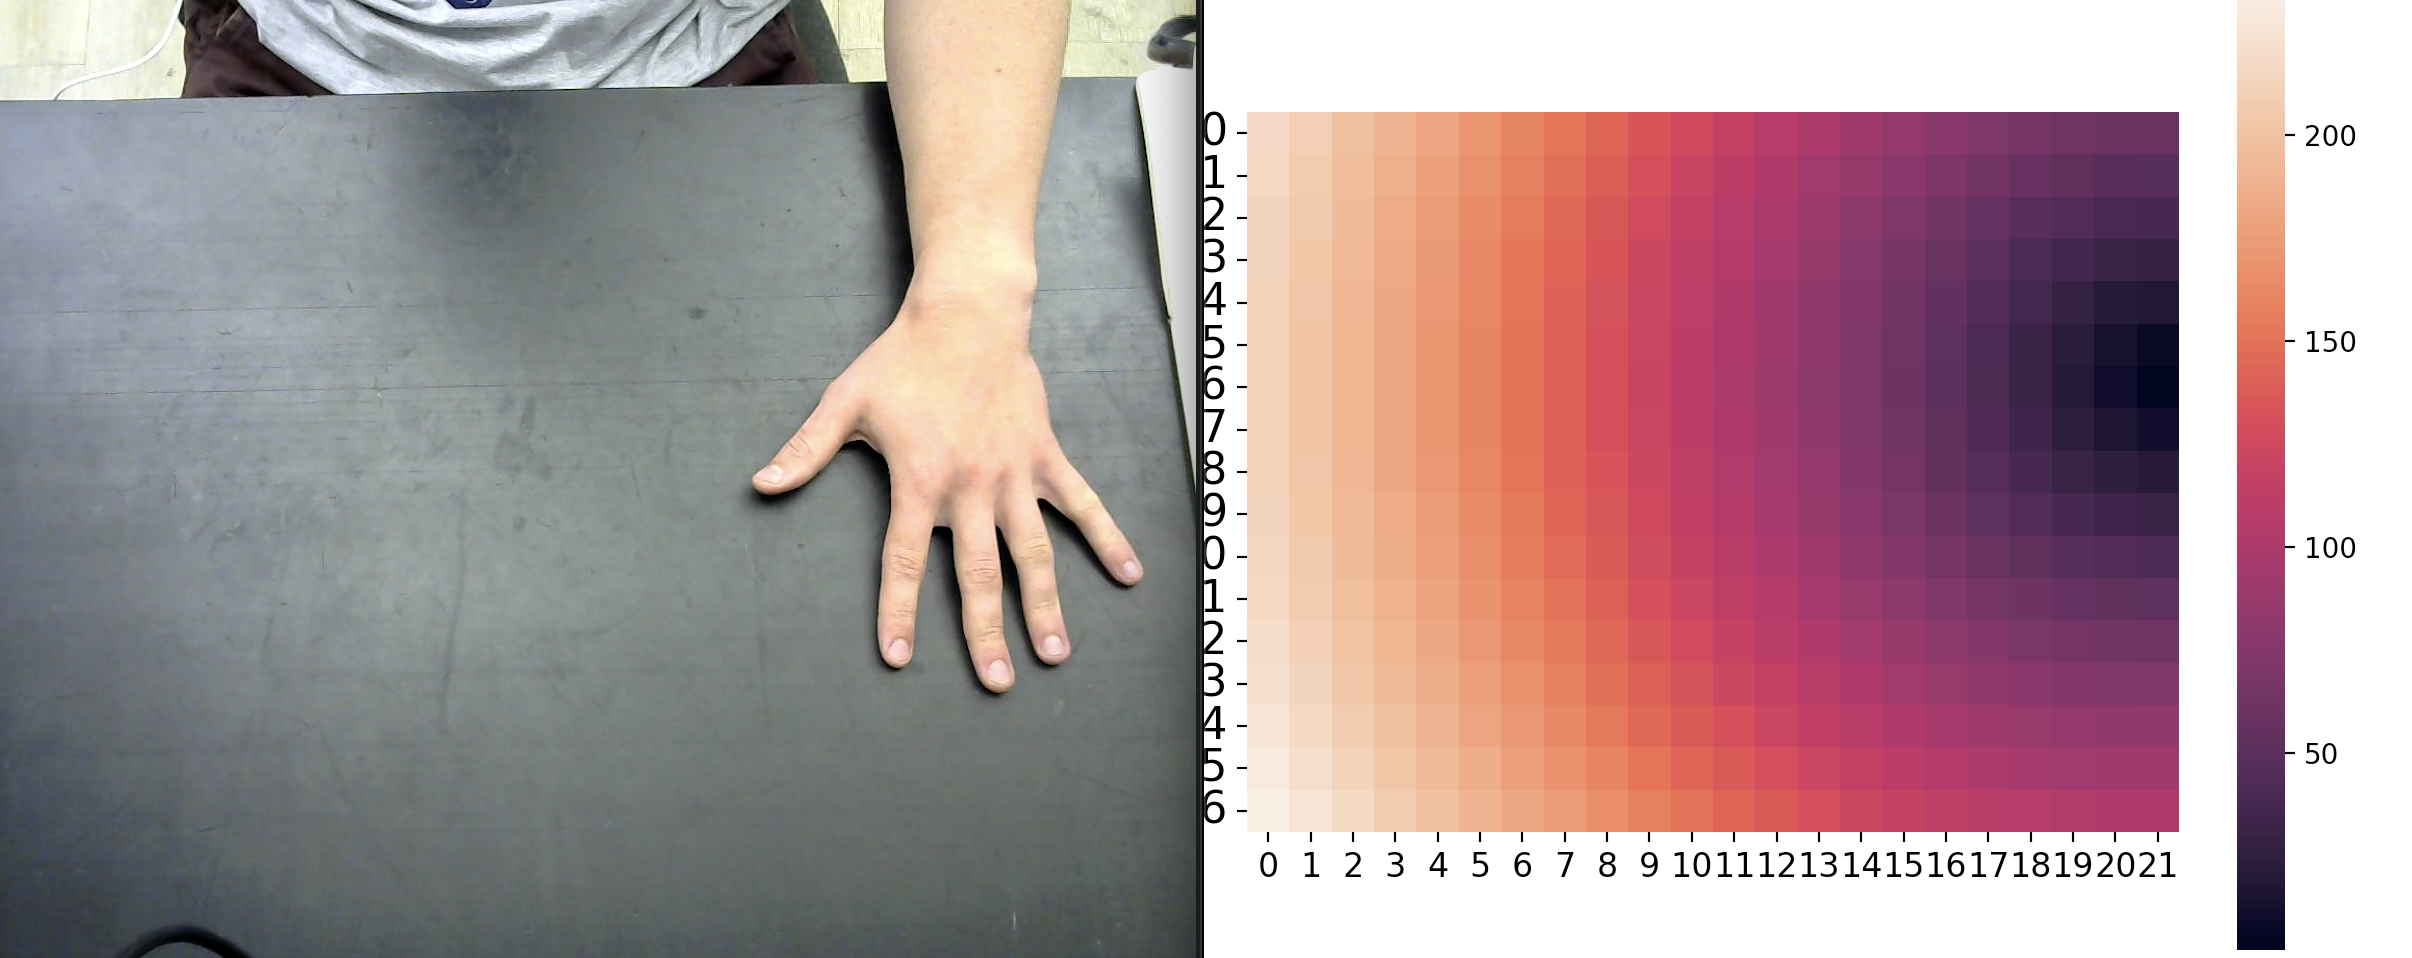
\includegraphics[width=0.7\linewidth]{figures/heatmap_hand_detector.png}
    \caption{Heatmap of hand detector}
    \label{fig:heatmap_hand_detector}
\end{figure}

After much experimentation it was realised that the system architected above with the heatmap and delta values was incapable of being learned by a convolutional neural network in its current state. There is just too much complexity and not enough training data for the network to generalize that a specific point on the hand was representative of the 0 delta value and training just saw exploding loss values.

\section[2022/08/23]{Tuesday, 23 August 2022}

\subsection{Hand locator changes}

The aim of this session is to continue work on the hand locator and construct up-to-date prototypes using as many first principles components as possible.

Because the heatmap delta neural network architecture is not working as desired, a new method of detecting the hand was devised - using classical methods. The mask of the Ycbcr-segmented image clearly shows a concentration of white pixels where the hand is located. By creating a number of candidate regions split across the image and looping through each region and summing the pixel values there, the general location of the hand can be identified. This is visible in the prototype constructed in \FigRef{fig:hand_detection_first_principles}. The system is mostly accurate except for when other large patches of skin are visible in the frame and when the hand in the frame is contorted in different manners. \\

Since the camera is in a top-down orientation, the user's arm will always enter from the top of the video frame. Thus finding the largest region of skin-coloured pixels nearest to the bottom of the screen will effectively account for error and will not detect the large part of the forearm instead of the hand. This was implemented by calculating a south delta value for each region which corresponds to its distance from the bottom of the screen. Finding the smallest value in this list gives the southern-most region of skin pixels in the frame. Finding the largest region of skin pixels within a certain range of this southern-most point yields the hand or palm region consistently. Thus the hand tracker is complete and will be left as is for now.

\begin{figure}[h]
    \centering
    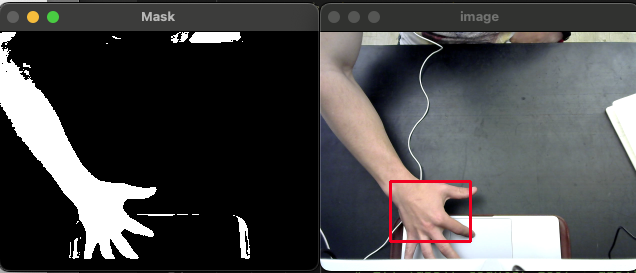
\includegraphics[width=0.7\linewidth]{figures/hand_detection_first_principles.png}
    \caption{Hand detector using mask concentration algorithm}
    \label{fig:hand_detection_first_principles}
\end{figure}

\section[2022/08/24]{Wednesday, 24 August 2022}

\subsection{World Coordinate System}

The aim of this session is to plan and prototype the world coordinate system.//

In order to have meaningful interactions between virtual objects and real objects a shared coordinate system must be established. This can be in the form of an x and y coordinate - being the width and height values of the input image as well as a depth value. The Kinect sensor outputs values between 0 and 2047 representing how far away a specific pixel is from the camera and thus giving virtual objects this coordinate too and growing/shrinking them according to this value will make sense. The planning for said system is visible in \FigRef{fig:kinect_world_coords_planning}.

\begin{figure}[h]
    \centering
    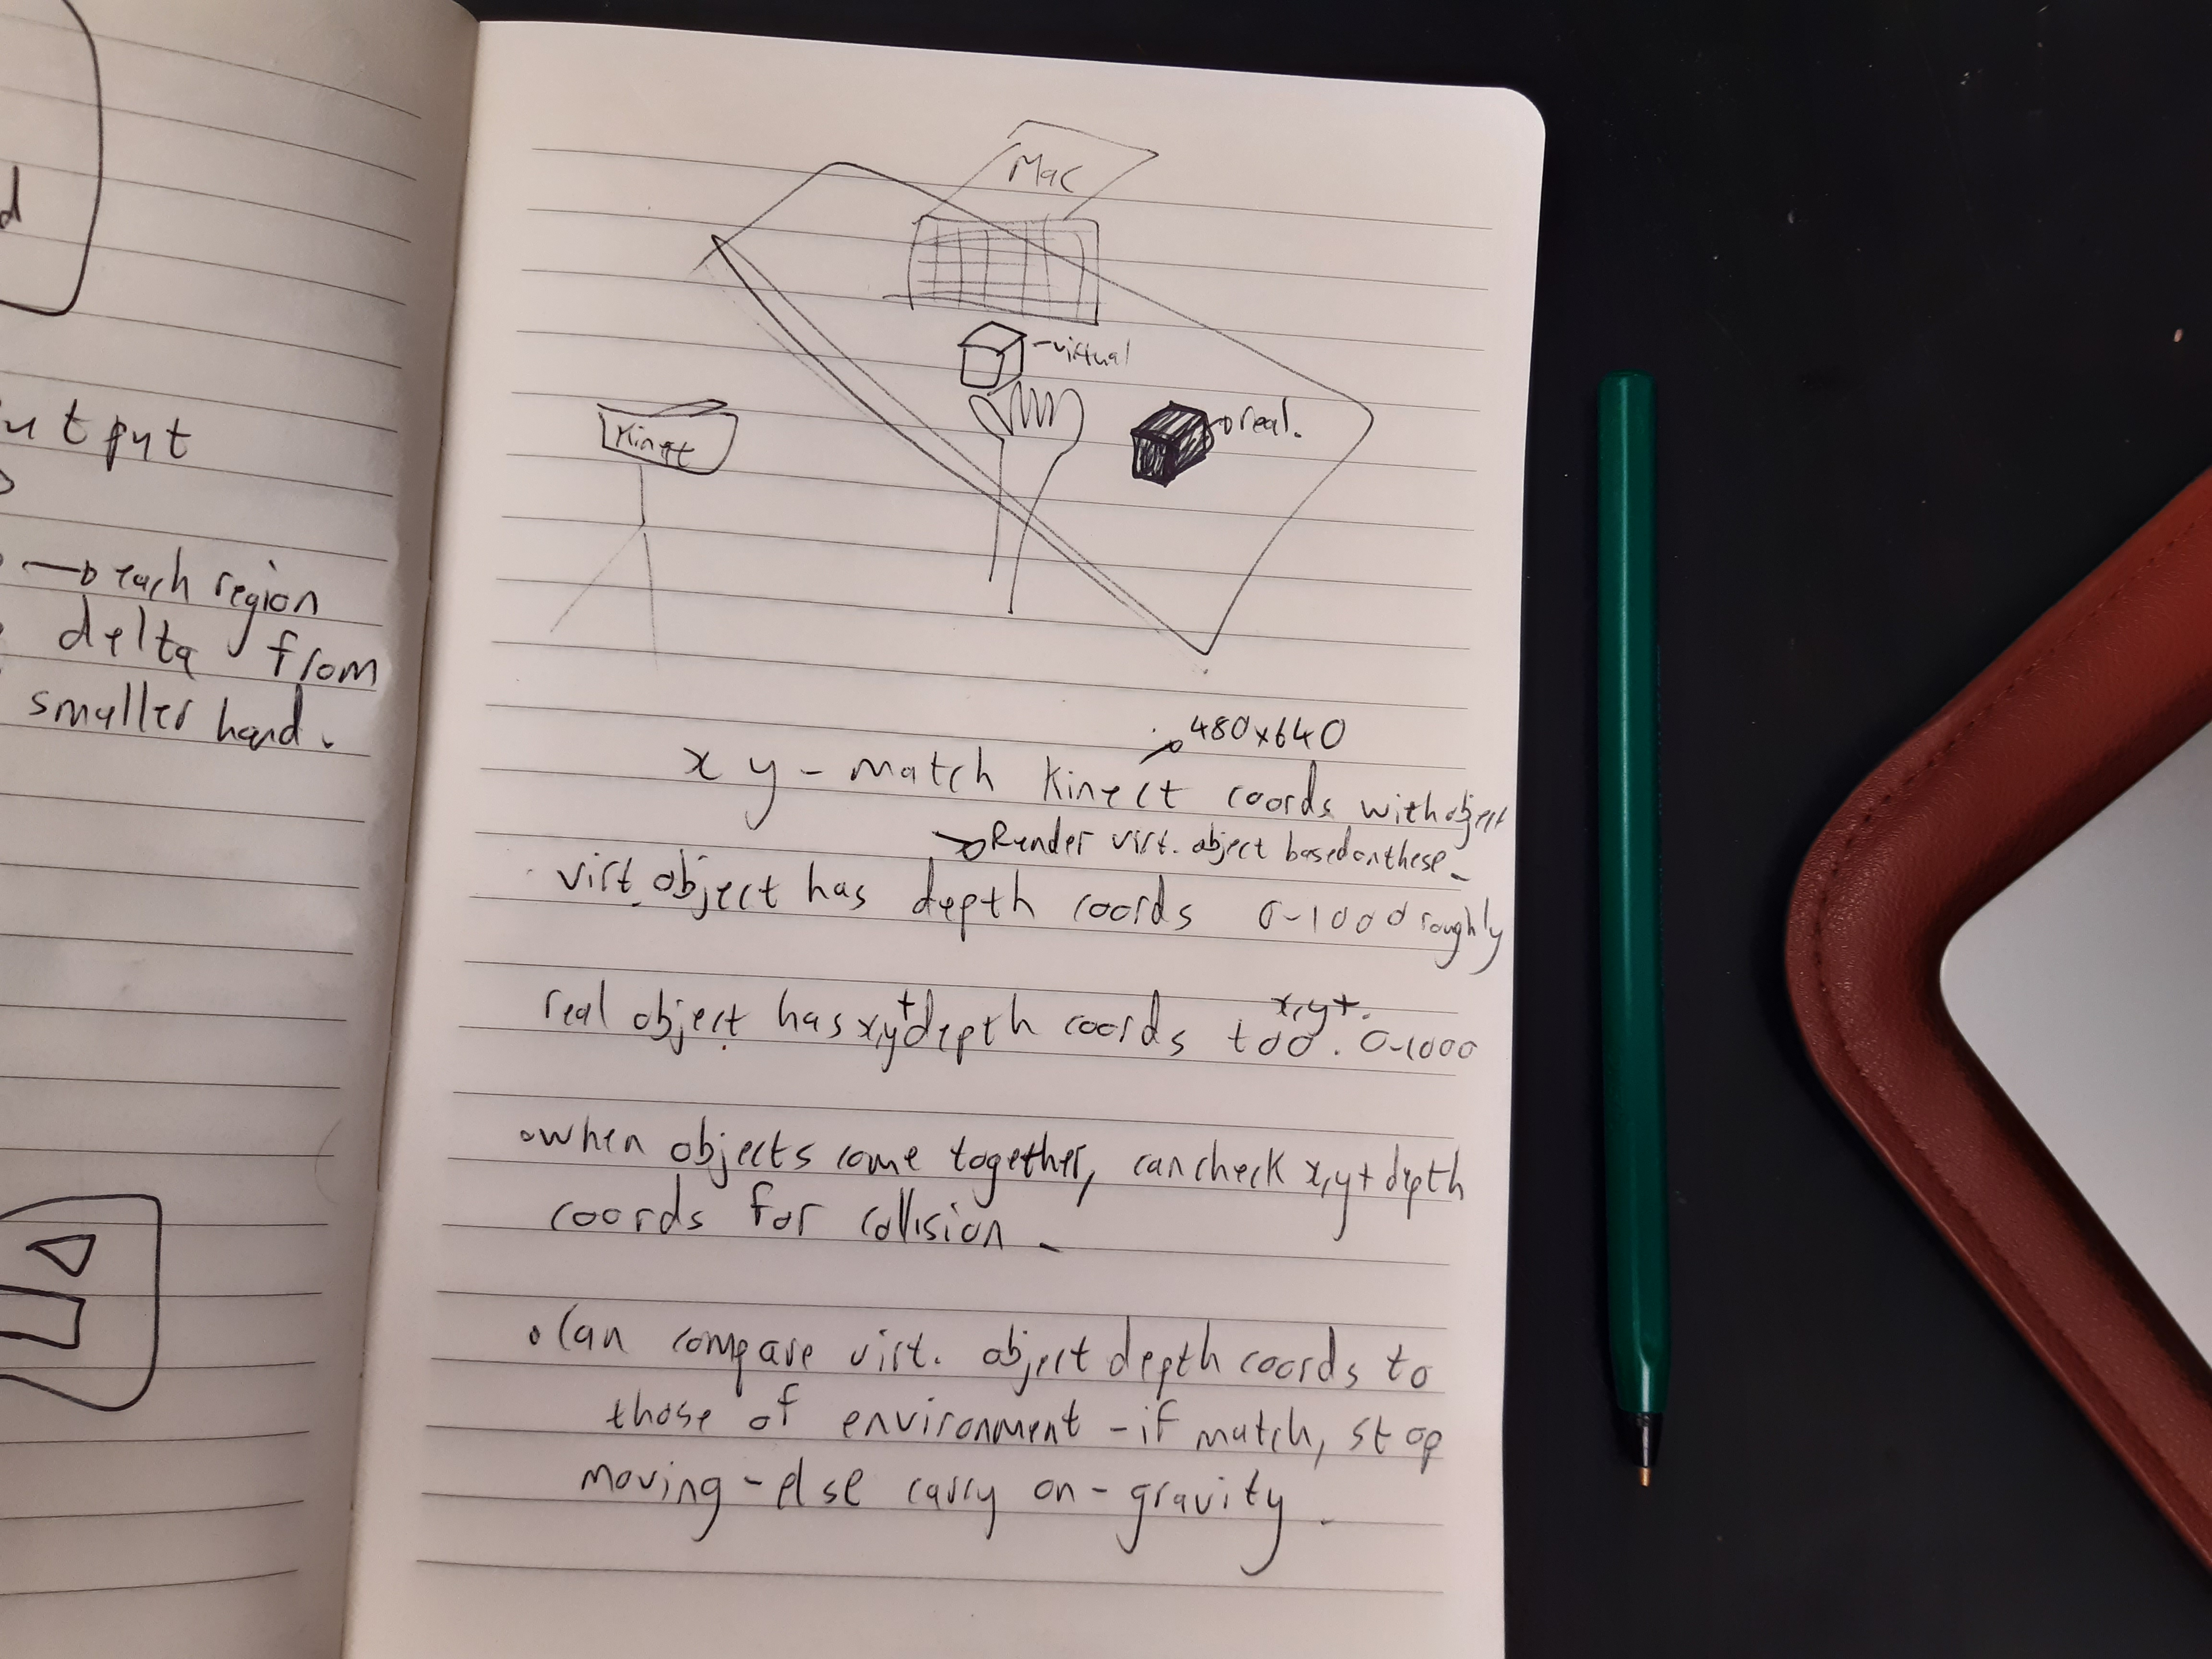
\includegraphics[width=0.7\linewidth]{figures/kinect_world_coords_planning.jpg}
    \caption{Planning of the Kinect and virtual object coordinate system}
    \label{fig:kinect_world_coords_planning}
\end{figure}

\section[2022/08/25]{Thursday, 25 August 2022}

\subsection{Virtual Object Rendering Changes}

Using OpenGL was initially decided upon because it was the industry standard for 3D graphical applications. However, interfacing the projection-based three-dimensional coordinates system with the two dimensional xy coordinate system used by the Kinect and ordinary webcams has proved challenging. In order to aid further development of the virtual object prototyping system, a prototype was constructed for rendering a virtual cube using OpenCV - which shares the same two-dimensional xy coordinate system as the Kinect. Building this prototype requires manually specifying each vertex of the cube in two dimensions and then rendering three distinct polygons which are the three visible faces of the cube. This is demonstrated in \FigRef{fig:OpenCV_cube_rendering}. Further prototyping will be needed to enable the cube to be rotated and generalized to any point on the xy coordinate system but it has removed a lot of transitional overhead for translating between coordinate systems.

\begin{figure}[h]
    \centering
    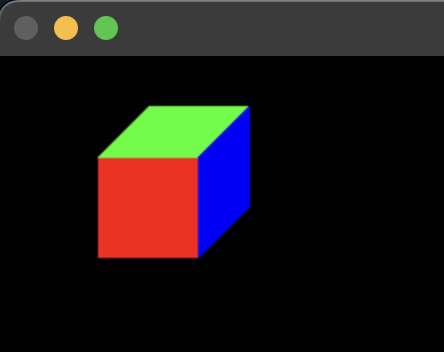
\includegraphics[width=0.7\linewidth]{figures/OpenCV_cube_rendering.png}
    \caption{Cube rendered manually using OpenCV}
    \label{fig:OpenCV_cube_rendering}
\end{figure}

The Kinect and OpenCV cube prototype were then combined in order to further prototype a collision avoidance system.

\section[2022/08/30]{Tuesday, 30 August 2022}

\subsection{Improvements to hand tracking and extracting}

Time was spent today on modifying the hand tracking algorithm to work with input from the Kinect sensor and a side-on view as opposed to a top-down approach since this is the desired use case of Mr. Grobler for the overall system - being able to reach into the scene and manipulate virtual objects there. The southmost delta calculations were modified to instead search for the largest region of skin-coloured pixels closest to the centre of the image as this is where the user's hand will predominantly be when interacting with the virtual object. More fine-grained control of the object is going to be necessary and so work turned to the open/closed hand classifier in Tensorflow.

A training data accuracy of 0.9798 and testing data accuracy of 0.9091 could be achieved with 120 input images. Data augmentation was performed and modifications to the network allowed this value to be increased to 1.0 and 1.0 on a small dataset of 240 images. Real-world performance is good and only in small edge cases such as when the hand is rotated to present a small cross seciton of a closed fist does the system classify the geture incorrectly - something that can be alleviated with tweaks to the network size and by introducing more training data. Thus this shows a positive step in using convolutional neural networks for the classifying of gestures and scaling this system up to more gestures is the next milestone. \\

The OpenCV cube prototype was connected to the improved hand tracking application and the cube could be moved around in the direction reasonably of the user's hand motions. Time was spent also considering how to mount the Kinect on a tripod for use in the final system - although it can actually just sit on top of a tripod the use of zip ties or another material to ensure the Kinect doesn't topple to the ground if the tripod is nudged was also considered.

\section[2022/08/31]{Wednesday, 31 August 2022}

\subsection{Hand directions neural network}

The aim of this session is to build a prototype hand direction classifier.


In order to control the virtual object a model of the hand needs to be identified at each time instance. This need not be a super high-fidelity model as the object just needs to be moved around the screen and rotated in a few directions. Thus building a classifier that can differentiate between a few directions of hand movement might be sufficient to control the object - testing will need to be conducted. A neural network is constructed to predict if a hand is facing left, right or upwards and is visible in \FigRef{fig:hand_direction_NN_first_attempt}. The system can accurately classify up and right when using the left hand as input and up and left when using the right hand - the system is learning wrist positions in the background and thus incorrectly classifying gestures when the hand is contorted to point in the same direction as the arm. This will need to be rectified in future implementations.

\begin{figure}[h]
    \centering
    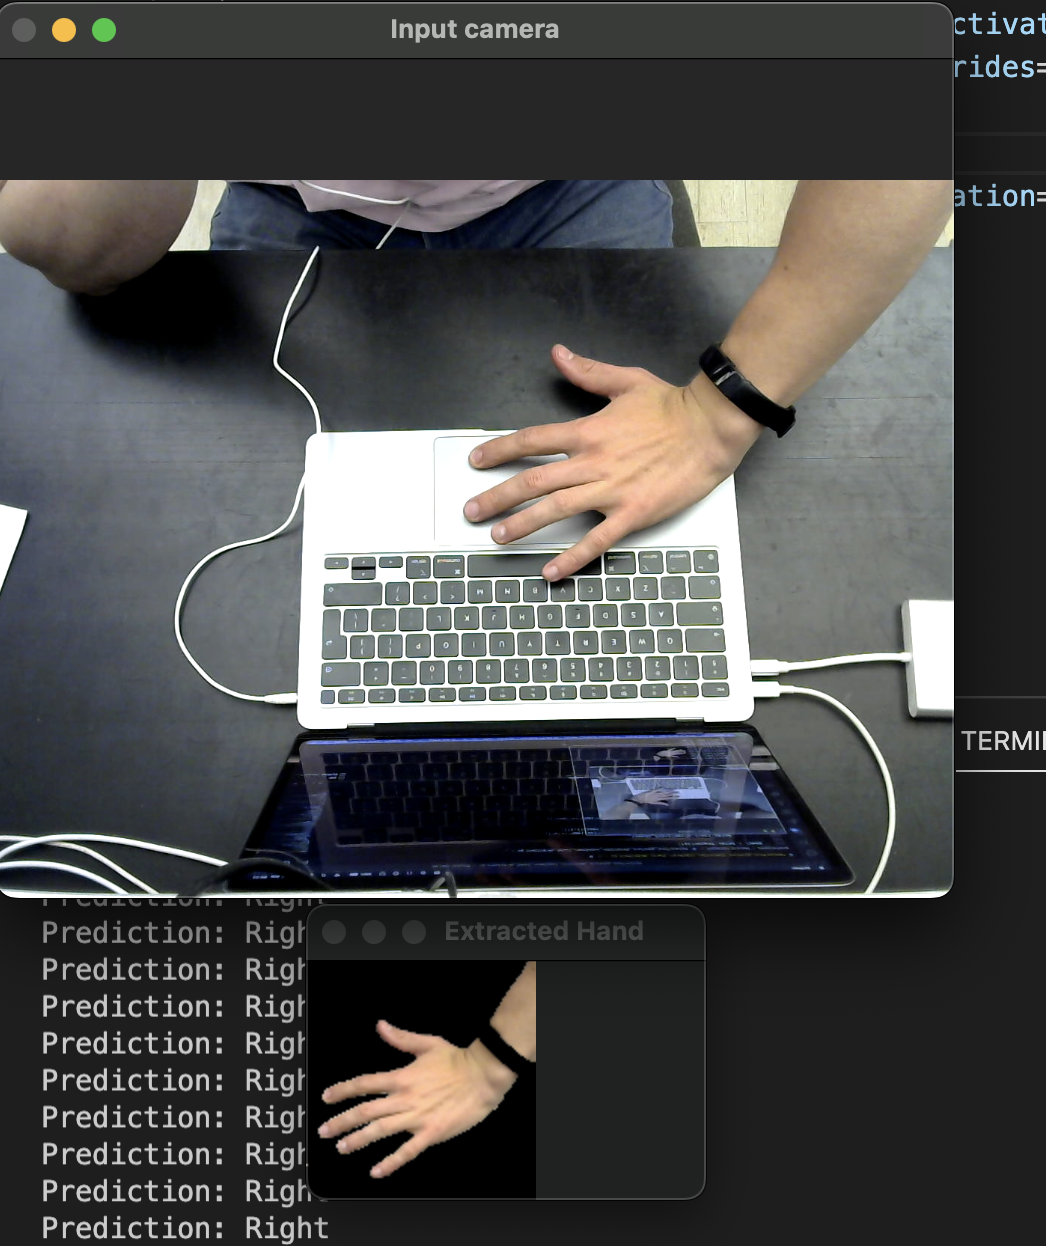
\includegraphics[width=0.7\linewidth]{figures/hand_direction_NN_first_attempt.png}
    \caption{Hand direction prediction}
    \label{fig:hand_direction_NN_first_attempt}
\end{figure}

In order to have an up to date prototype system the top-down open hand/fist classifier is combined with the OpenGL cube rendering code so that when the user has an open hand nothing happens but when they make a fist and "grab" the object it begins to follow their hand as if they had picked it up. The implementation is visible in \FigRef{fig:OpenGL_tensorflow_open_hand_fist_grabber}.

\begin{figure}[h]
    \centering
    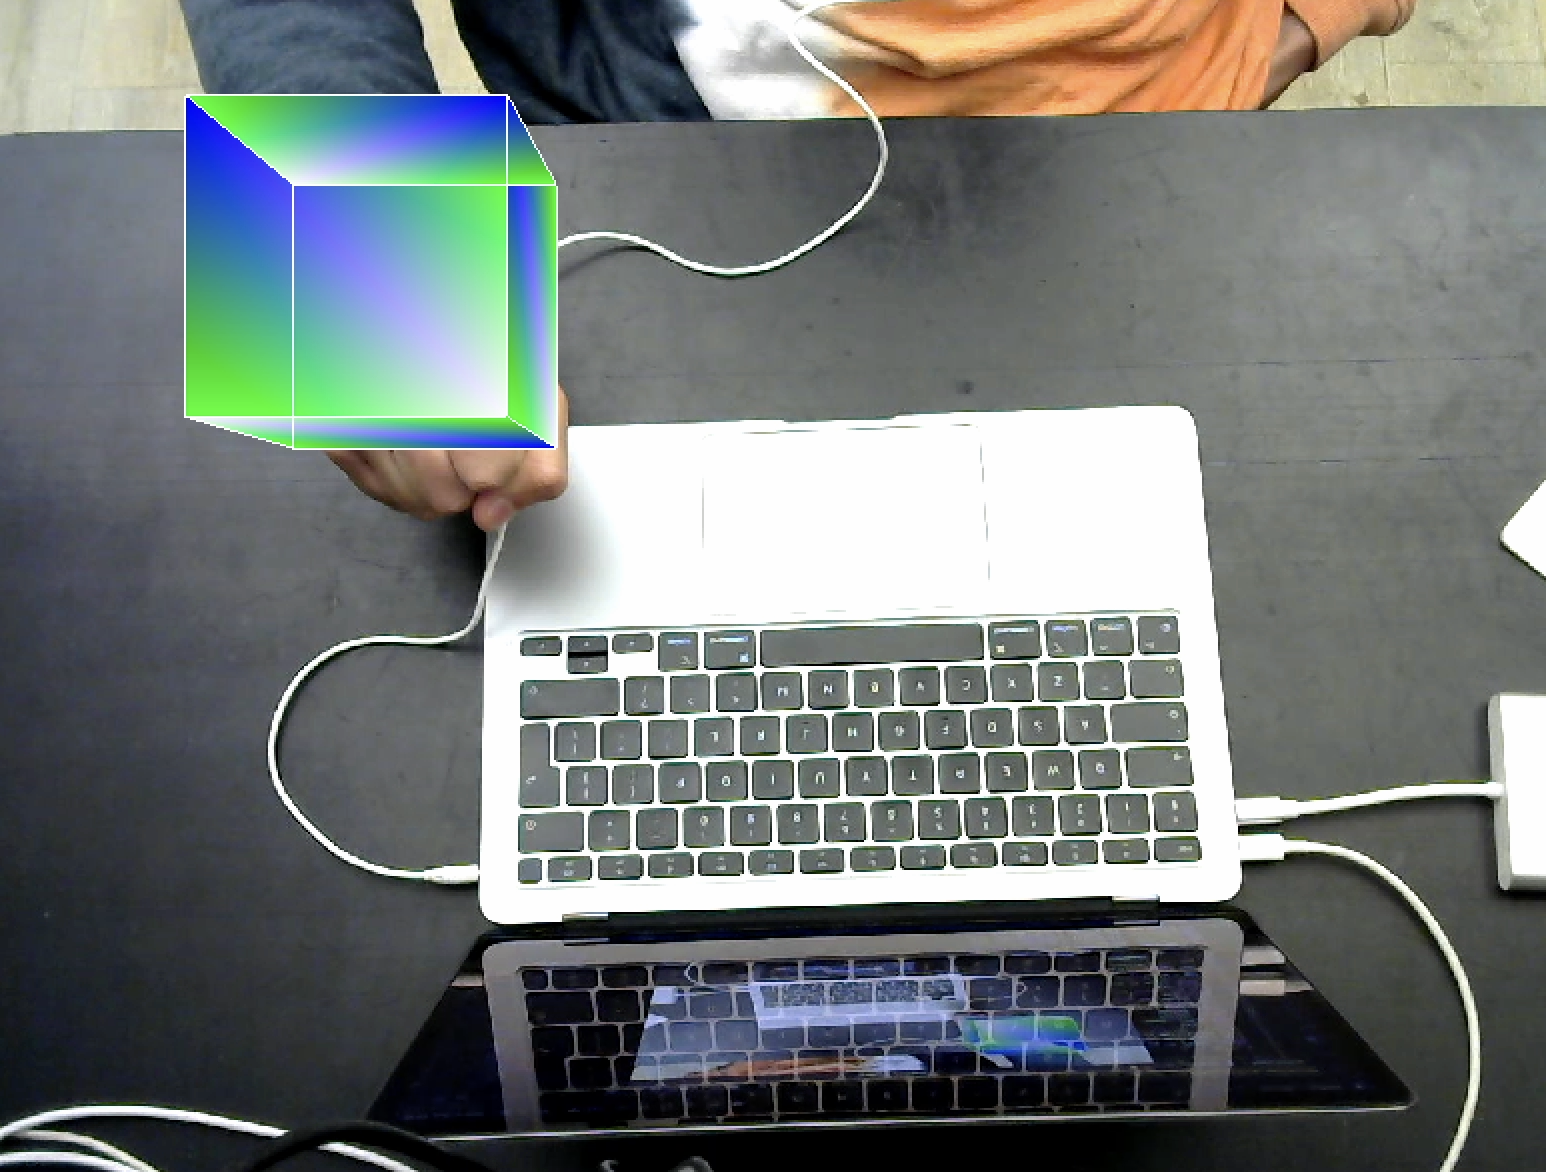
\includegraphics[width=0.7\linewidth]{figures/OpenGL_tensorflow_open_hand_fist_grabber.png}
    \caption{Top-down cube grabber prototype}
    \label{fig:OpenGL_tensorflow_open_hand_fist_grabber}
\end{figure}

